\chapter{Programmable Computer Networks}\label{sec:ch-networks}\label{chap:nets}
Computer networks serve the important function of allowing any two machines to communicate with one another, typically via individual messages know as packets (i.e., a packet-switched network).
Naturally, reality is much more complex than this broad statement would otherwise let on; the local routing fabric in a modern network comprises specialised (though commonplace) hardware for correctly routing these packets through arbitrary topologies of links and switches at ever-increasing data rates.
This grows more complicated still when we consider the task of \emph{inter}networking between such networks, where we must route packets on higher-level logically structured addresses between different domains of control according to fairly complex policies and relationships.
At the inception of these technologies, computer scientists of the day wisely decided that the sole duty of the network itself should be the correct routing of individual packets.
Their view was that application-level logic should be executed solely at endpoint machines; their definition extended, of course, to even include desirable (and some would say indispensable) transport-level properties such as error checking and stream reliability.
This is known as the \emph{end-to-end principle}~\parencite{DBLP:journals/tocs/SaltzerRC84}.
This position arose partly due to the logical complexity of all the tasks pushed onto the network at this time, as well as the need to ensure optimal forwarding performance while microprocessors were still relatively nascent, but was instrumental in ensuring that the network itself remained \emph{extensible}.
A consistent, pared down feature set ensured while offering a good degree of freedom for the development and deployment of higher-level protocols.

Decades have passed since then, and to a large extent the zeitgeist has shifted on just how capable our networks should be---in both the research community and operators of large-scale networks.
Consider the case where an operator has a fully converged network built entirely on fixed-function hardware, but wishes to use some program to inspect the behaviour, state, and characteristics of some flow between two local machines.
The problem is that these devices offer no means of modifying or influencing routing state, being highly-optimised switching devices that understand a selection of routing algorithms built into their internal circuitry.
For the longest time, altering the network's routing behaviour in this instance---even for a single override---required not only physically altering and rewiring the network, but also would require additional hardware.\sidenote{Revisit this later... maybe a better example will come to me?}
\gls{acr:sdn} was a key development in enabling this fine-grained routing over traffic at various layers in the protocol stack, allowing operators to offer per-flow or per-class routing for improved performance---\gls{acr:te}---or even application-aware load balancers at the switch level.
Initial forays into \gls{acr:sdn} were built on the exploiting a separate \emph{control plane}, which would install \glspl{acr:mat} on target switches---mapping fields of predefined protocols to predefined actions---leaving truly complex decisions to one or more controller machines.
These developments have been pushed even further as the runtime capabilities of supporting devices have evolved into what we might now consider truly \glsxtrfullpl{acr:pdp}.
A wide variety of \glspl{acr:asic}-based switches, SmartNICs, and other accelerators now offer an environment for truly arbitrary network logic, protocol parsers, and action definitions.

Despite all this, our general-purpose Internet remains much the same from an endpoint perspective, performance and reliability increases aside.
Yet this increase in capabilities has revealed new strands of research in more specialised networks such as those in datacentres, where in-controller processing would have allowed the network fabric to \emph{cooperate} with its hosted applications but presented an obvious computational bottleneck.
\emph{In-network compute} is enabled by such bespoke routing environments such as theirs when combined with the above advances in programmability.
In-network compute is founded on the growing idea that in-path network elements such as switches, \glspl{acr:nic}s, and middleboxes can and should act as the site of complex logic to accelerate applications, participate in flow control, or to aid in network management.
%In this field
%
%?? Talk about application benefits.
%?? In-network compute.
%
%Of course, over the last 
%?? Levels of engineering work at many levels of abstraction which interlink, interlock, and depend on one another
%
%What we have now are a wide variety of ways to run programs of varying levels of complexity at ?? many levels of the stack ?? to aid application and networkr performance

In this chapter, I'll...
\section{From Fixed-Function to Fully-Programmable}

?? What are networks?

?? Possibly discuss the internet

?? Lead in from ARPAnet et al. (2 paras). Scientific comms -> general use,

The intro of choice~\parencite{DBLP:journals/ccr/FeamsterRZ14}

?? interconnection physical and reconfig are main challenges that made SDN look attractive, reasonable?

Control plane programmability: routing etc? Dataplane programmability: per-packet computations.
?? focus on programmable \emph{dataplane} rather than control plane

Programmability in computer networks tends to be categorised into two distinct forms.
\emph{Control plane} programmability focuses on the routing of packets, making it easier to alter, update, and tailor the forwarding behaviour of a network at run time, and at many levels of granularity.
?? Programming the \gls{acr:fib}/\gls{acr:rib}
\emph{Dataplane} programmability focusses instead on introducing additional logic into the network to be executed by the forwarding elements such as routers---stateless or stateful transformations of packet streams, traffic measurement, and so on.
There is, of course, vast scope for their interaction. ?? describe

\subsection{Active Networking}\label{sec:active-networking}
In response to the expanding scale and widespread reach of the Internet (and computer networks in general), researchers in the early-to-mid '90s increasingly desired the tools to extend, innovate, and research routing and transport protocols.
To maintain and safeguard interoperability over the Internet, the \gls{acr:ietf} formed to maintain and oversee the development of Internet protocols for all levels of the networking stack.
The weight of full \gls{acr:ietf} standardisation was seen by many researchers of the period as a lengthy process, which they believed to be the cause of \emph{network ossification}---the Internet becoming inflexible to the design and deployment of new protocols.\sidenote{Authors of this period might be horrified to discover that the \gls{acr:ietf}'s median time to standard publication has more than doubled since 2000~\parencite{DBLP:conf/imc/McQuistinKKPTPH21}. This is not, however, what we understand as ossification in today's Internet, which I'll discuss shortly.}

\emph{Active networking} was researchers' response: a family of clean-slate proposals built around enabling switches to perform arbitrary computations on carried packets, and for the network to share resources such as compute and memory with users and applications~\parencite{DBLP:journals/ccr/TennenhouseW96,DBLP:journals/ccr/Calvert06}.
This is a more communistic, cooperative view of the role of the network---that it should provide and manage advanced services as a sort of common good beyond raw forwarding capacity and functionality, more than simply `best-effort'.
%Shared resources, expectation of the network to `do something'.
This would enable not only new protocols empowered by the cooperation of the routing fabric, its proponents argued, but would also simplify network management and measurement; it was in no uncertain terms a radical departure for its time, standing in stark opposition to the simplicity demanded by the end-to-end protocol.
Active networks planned to enable cacheing and \gls{acr:cdn}-like behaviour, stream compression, network management, and telemetry.

Surveys of today divide the ideas of this movement into two main streams of research~\parencite{DBLP:journals/ccr/FeamsterRZ14}:
\begin{description}
	\item[Capsules,] which consisted of compact programs bundled inside of network packets; either at a per-packet level, or installed on a per-flow basis during the handshake process.
	\item[Programmable switches,] which allowed arbitrary programs to be installed by system administrators to their own infrastructure for dataplane processing.
\end{description}
These are two key tools rather than opposing schools---and works we'll examine from tail end of the \emph{active networks} movement feature a high degree of interplay of both ideas.
It must be said that in the absence of specialist supporting hardware, the vast majority of works in this field relied entirely upon execution of high-level code via commodity host machines.
\gls{acr:udp} tunnelling and overlay networks like \emph{PlanetLab}\sidenote{PlanetLab also had a wider effect on distributed systems research. Sadly, it was shutdown in May of 2020~\parencite{planetlab-rip}.}~\parencite{DBLP:journals/ccr/ChunCRBPWB03} were necessary to do so; the former modelling a cooperative multi-\gls{acr:as} Internet in a testbed setting, and the latter providing hosts with \gls{acr:cpu} and memory slices across the world in a ticketed, quid-pro-quo manner.

\paragraph{Innovations in capsules}
\emph{ANTS}~\parencite{ANTS,DBLP:conf/dance/Wetherall02} captured the (almost stereotypical) active networking idea of `arbitrary user programs' selected by each packet.
A capsule contains one or more program IDs in each header's packet, to be inspected by an ANTS runtime at on-path active nodes.
Capsules include dataplane programming and routing logic, kept immutable between flows.
An active node checks its local cache for program code matching a capsule's IDs, which may be pre-installed by an administrator (out-of-band); on a cache miss, the code is requested from the last active node (in-band).
Programs for a given ID are verified and signed externally by some trusted organisation e.g., the \gls{acr:ietf}, but their use is still controlled by \emph{the user or endpoint application}.
%?? in-band and out-of-band installation: pre-install or request prog from prior hop on miss.
ANTS relied on the transfer of Java code: extensions such as \emph{PAN}~\parencite{PAN-activenet} investigated the use of raw unsafe x86 assembly for, e.g., in-kernel use.

\emph{Smart packets}~\parencite{DBLP:journals/tocs/SchwartzJSZRP00} examined dataplane programming from the perspective of measurement and control.
Intended as a means for management centres to install packet programs on managed nodes, one or more initialisation packets would be sent across the network between a source and destination---each containing a single complete program and all relevant authentication certificates.
Any nodes along the path---including endpoints---would be free to install or pass on logic as required.
Programs were limited, stateless, compact programs executed in a \gls{acr:vm} for all carried packets, with dedicated intrinsics for accessing state from the \gls{acr:mib}; packets could trigger \gls{acr:mib} events, or modify a packet to include per-path telemetry supporting passive and active measurement use cases.
Hosts and switches were expected to enforce limits on execution time and dynamic memory use.

\emph{NetScript}~\parencite{DBLP:journals/jsac/SilvaYF01} allows for the definition of active network programs as a dynamic (i.e., potentially branching) dataflow graph of smaller programs---\emph{boxes}.
Such boxes may be recursively defined.
Crucially, its main advantage over the similar \emph{Click}~\parencite{DBLP:conf/sosp/MorrisKJK99} is that any box can be a remote node (another machine, or a specialised hardware/\gls{acr:asic} implementation), which makes this a remarkably prescient combination of control plane and dataplane programmability.
Dataplane program definition and selection is left entirely to network operators in this abstraction, however.

\paragraph{Switch programmability}
Though conceptually purer uses of programmable switches are rarer, their use is often implicitly assumed to be necessary in any real, performant active network.
The \emph{SwitchWare} project~\parencite{DBLP:journals/network/AlexanderAHKKMG98}, while very much a capsule-based proposal, primarily suggested a base of \emph{SANE}-backed switches~\parencite{DBLP:journals/network/AlexanderAKS98} which would implement a fixed, performant set of `active extensions' analogous to \gls{acr:os} syscalls.
Ahead-of-time fixed subprograms like these were key here to achieve performance and security---mainly by limiting capsule program capabilities and allowing delegation to, e.g., \gls{acr:asic} accelerated operations.

From a more practical perspective, \Textcite{DBLP:journals/jsac/WolfT01} examine the design requirements of a programmable switch in contrast with emerging \glspl{acr:npu} of the time.
They propose a \gls{acr:soc} design built around a large array of general-purpose \gls{acr:risc} \glspl{acr:cpu}, each having their own cache and memory.
A first stage \gls{acr:asic} would route packets to an output port over a shared interconnect, where these \glspl{acr:cpu} would either count as their own port or be attached to a physical egress and conditionally used.\sidenote{Curiously, this design more closely matches modern SmartNIC devices, while today's programmable switches favour \gls{acr:asic} designs. We'll return to this point in \cref{sec:modern-pdps}.}
The inclusion of complete \gls{acr:risc} \glspl{acr:cpu} is quite deliberate: early \glspl{acr:npu} such as the Intel IXP1200~\parencite{intel-ixp} and Lucent's Fast Packet Processor~\parencite{lucent-fpp} had unusual instruction sets suited to stateless processing of headers~\parencite{DBLP:conf/pldi/GeorgeB03}, limiting their general expressiveness.
A fuller \gls{acr:isa} was recognised as being necessary for more capable, general, useful, and stateful dataplane programming; particularly of the kind envisioned by active networking.

%, which is where perf-router cite succeeds. ?? stateless etc.

%?? mention smartpackets's exec model here.

Returning to \emph{smart packets}, we see a similarly earnest attempt to reconcile capsule networks with a reasonable, programming framework (as opposed to its peers' focus on high-level languages).
Aiming to be more amenable to switches they propose \emph{spanner}, a compact \gls{acr:cisc} assembly language for a stack-based \gls{acr:vm} with primitives to access the \gls{acr:mib}, compiled to by their own higher-level language.
Spanner was designed to be reasonably implemented on hosts and routers, but explicitly trades performance for compactness, focusing on small, self-contained, stateless and secure programs.\sidenote{This shares many conceptual similarities to \gls{acr:ebpf}, a \gls{acr:risc} register machine, which now plays a key role in network compute offload and \gls{acr:os} kernel extensibility. The \gls{acr:vm} abstraction, using intrinsics and maps to communicate with the environment, ensures security while the language's simplicity allows implementation in the network fabric.}
The executing switch or host enforces memory and execution limits at runtime, but single-packet $\mathcal{O}(\text{\qty{1}{\kibi\byte}})$ programs simplifies deployment logic.
Naturally, this excludes stateful boosters of the type we've examined, but is well-suited to the measurement and management use cases its authors intended.
%?? HLL -> \gls{acr:cisc} Assembly for stack-based \gls{acr:vm}\sidenote{}, with primitives to access \gls{acr:mib}. Focus: small, self-contained, stateless secure.

%?? Tie into PDP here: active networking and TPP . Think about the concept of protocol boosters~\parencite{DBLP:journals/jsac/FeldmeierMSBMR98}. (NOT READ)

\paragraph{Failings and drawbacks}
Sadly, the active networking paradigm failed to properly fledge, at least in its first iteration.
It might be argued that the `communistic' network view played a key part in this downfall---that the tangled web of \glspl{acr:as} between any two nodes should freely offer compute resources to the benefit hosts.
This comes down to a simple question of economics: who pays whom for providing these services?
It's easy to reason about this in campus or internal networks (the organisation provides active capabilities as part of its own remit), or if we require that only our \gls{acr:isp} offers these capabilities (hosts pay for them explicitly).
Extending this notion to the wider Internet becomes more challenging.
Assigning responsibility for administrative, technical, and security issues among all the organisations between two endpoints is a daunting prospect, to say the least.
When modifying packets in a protocol booster-like model, it becomes difficult to communicate where boundaries of support start and end to enable truly transparent behaviour.
In a setup like the PlanetLab overlay network the incentives for providing these capabilities in such a distributed way are obvious: all the users are researchers in need of distributed network compute.
Each benefits from donating compute and network slices in their own infrastructure to receive resources in kind.

The problem here is also one of aggregation.
At the Internet core such as in \glspl{acr:ixp}, transit bandwidth demands are the sum of all connected \glspl{acr:as}, amplifying compute demands and scale concerns.
From another angle, suppose that all functions benefit the network \emph{and} hosts alike, as in the case of an in-band \gls{acr:tcp} compressor.
Here, files can be transmitted between end hosts quicker \emph{and} the bandwidth impact on the switching fabric is reduced.
If hosts benefit and have the resources to implement this functionality it is inevitable that at some point they will do so (pushing logic to the network edge), at which point network operators are able to put their own resources into faster or higher-capacity passive infrastructure with a vastly reduced attack surface compared to an active solution. 
On the upside, this also preserves the end-to-end principle.

% is part of its downfall administrative, tech, security issues etc. Even though some use cases would have benefited admins (i.e. compression to expand capacity).
%?? Obvious in PlanetLab: incentives are all users are researchers!
%?? Lots of economic drivers: who pays whom for providing these services? Why not just push this logic to hosts (preserving end-to-end) if the logic (i.e. compression) benefits the network AND hosts too?

%?? More issues? complexity, where boundaries of support start and end (and how to communicate them) (for instance, in protocol boosters).
%?? Flow migration and redundant failover, and path aggregation far harder?
%?? In ANTS, implications for flow buffering on prog miss.

Active network capabilities do in many senses \emph{limit} how networks can benefit their users (or at least make some innovations substantially harder).
Consider flow migration, potentially as part of a wider \gls{acr:te} strategy, or path aggregation to increase bisectional bandwidth or provide redundancy to protect from link failures.
Administrators must not only handle routing and design of such capabilities, but they must also ensure that active network programs on any flow's path are mirrored or migrated to the new path.
In the event of a complete or partial node failure, this may not be trivially possible.
Even when retrieving programs from the last hop, failover may be needed for a live high-bandwidth flow, requiring costly per-flow buffering at a node until capsule program setup is complete.

The capabilities of programmable network hardware were, to some extent, overshadowed by the community's focus on the more intoxicating idea of capsule networking.
Naturally, the overwhelming majority of these platform were prototyped on host machines, which limited forwarding and processing performance far below that of even the reduced Ethernet line-rate of their time.
The repeated emphasis on high-level prototypes reduced the focus on the sorts of low-level, capable languages a performant system would require---proposals were instead marred by in-vogue high-level \gls{acr:vm}-based languages such as Java and Caml, which didn't do credibility any good.
This likely added to industry scepticism---one gets the sense of a paradigm driven by research trends instead of limiting its own boundaries to produce something truly capable and scalable.

\subsection{Software-defined Networking}
In parallel, a good many researchers saw a need to innovate (and fight stagnation in) the space of what we now understand as control plane programmability: the ability to deploy and develop new routing protocols, provide bespoke routing for individual packets, flows and applications, and to adapt to changes in the network itself.
While likely starting out from the same perspective as active networking---enabling new capabilities and development, and network evolution---as years have gone by greater network capacities, usage demands and a need for far greater reliability have introduced challenges manyfold.
Greater capacities, particularly in bisection bandwidth, typically mean more equipment for network admins to manage through routers and switches, but also in terms of additional cabling for link redundancy and aggregation---neither of which play well with older spanning tree protocols.
\glsxtrfull{acr:te}---making effective use of this capacity and providing different traffic classes with optimal forwarding---has similarly become more and more important over time.
The problem is that classical routing protocols such as \gls{acr:ospf} and \gls{acr:rip} are designed for distributed autonomy, offering no support for direct routing rule insertion by administrators.
Early \gls{acr:te} approaches were thus built on a shaky foundation of hacks and tricks, exploiting routing protocol behaviour to achieve the desired high-level outcomes~\parencite{DBLP:journals/ccr/FeamsterRZ14}.
Naturally, such workarounds become untenable and impossible to reason about at scale---particularly as failures and misconfigurations creep in and become harder to find and diagnose.
Effective though these early forays were, they remained hamstrung by the tightly coupled control and data planes of the network hardware of that era.
The reality and urgency of this problem space has led to the true separation of forwarding elements (the dataplane) from the logical control elements which inform and orchestrate their routing behaviour (the control plane).
This separation has enabled \glsxtrfull{acr:sdn}---the use of arbitrary machines and logic to define the forwarding behaviour of each and every network element~\parencite{DBLP:journals/comsur/NunesMNOT14,DBLP:journals/ccr/FeamsterRZ14}.
As we shall discuss, this has brought forth a well-developed and successful bevy of innovations in network control and design.

\paragraph{Development of the control plane}
This line of work began in earnest with the \emph{open signalling} movement~\parencite{DBLP:journals/ccr/CampbellKMV99} in \gls{acr:atm} networks, circa 1995, which aimed to standardise the \glspl{acr:api} and protocols for passing routing protocol data to its relevant handler (and rules back to line-cards)---in an era where these elements were still tightly bonded in commercial routing hardware.
\emph{Tempest}~\parencite{DBLP:journals/network/MerweRLC98} marked its zenith, using these capabilities in tandem with specific functions of these now-obsolete \gls{acr:atm} networks to define a `network control architecture' which would oversee correct forwarding policies and resource allocation.
Its primary focus, however, was in providing independent virtual network slices---\emph{switchlets}---to users of multi-tenant networks on demand, allowing these users to pass in their own control programs written for host execution in Java, for instance.
Control plane traffic from control elements to the dataplane was carried \emph{in-band} at this time (i.e., using the same fabric as tenants' datagrams).

%?? What do I want to cover? first: separation of ctl plane, OF and Net OSes (ONOS, OpenDaylight, ...), then bring around to vNFs etc
%
%Tempest~\parencite{DBLP:journals/network/MerweRLC98} for ATM networks, built on principle of \emph{open signalling}~\parencite{DBLP:journals/ccr/CampbellKMV99} (in ATM) from 1995. IP/Ethernet networks still `bonded' FEs and CEs in routing design.
%
%?? Greater capacity and use forced focus on \gls{acr:te}, which was onerous and required insane workarounds w/ fixed-fn hardware~\parencite{DBLP:journals/ccr/FeamsterRZ14}

These ideas were refined into general standardisation for hardware elements along a shared bus via \emph{ForCES}~\parencite{rfc3746}; stripped, of course, of the more visionary aspects such as network slicing, arbitrary control code, and wider resource management.
Primarily, this was focussed on registration of control plane elements, including key provisions for extensibility and discoverability to announce additional protocols and offer redundancy.
The move to physically remote control elements was proposed by \emph{SoftRouter}~\parencite{lakshman2004the}, such that forwarding and control elements would communicate with one another in-band over the same network they define (after a simple spanning-tree bootstrap phase) using custom discoverability protocols.
In particular this allowed its authors to experiment with reducing the number of control elements in a network, from which they observed faster convergence of protocols such as \gls{acr:ospf}.
Hardware capabilities did not at this point allow this level of control, and as such host-based routers like \emph{XORP}~\parencite{DBLP:journals/ccr/HandleyHK03} (dataplane in kernel, control plane in user space) and simulators such as \emph{ns} reigned in research at this time.

While most of the above work focusses on the \emph{intra}-domain case---routing \emph{within} an \gls{acr:as}---RCP~\parencite{DBLP:conf/nsdi/CaesarCFRSM05,10.1145/1016707.1016709} was instead motivated by how \emph{inter}-domain routing \emph{between} \glspl{acr:as} might benefit from the sorts of centralised control we now associate with \gls{acr:sdn}.
The problem in this instance is that edge routers must understand and implement \gls{acr:bgp}, each having their own arcane policies to achieve the intended network behaviour with respect to quirks of the protocol, their own hardware, and in the routes forwarded by neighbouring \glspl{acr:as}.
Their solution was to centralise this logic into one (or a few) host machines, providing a drop-in solution which could act on \emph{all} gathered \gls{acr:bgp} information to produce optimal decisions with better scaling characteristics, reduce administrative overhead and fragility, and which opened the door to later extension if neighbour \glspl{acr:as} also deployed RCP.

With the growing need for \gls{acr:te} and \gls{acr:to} at various layers of the Internet infrastructure, we begin to see a drive for wider coordination in the intra-domain case.
\emph{PCE}~\parencite{rfc4655} is one of the first serious attempts to formalise a network architecture where the control plane can calculate and install bespoke \emph{paths} at the flow level, given any set of constraints.
Naturally, this requires far greater coordination of the individual forwarding behaviour of switches, preferably combined with \gls{acr:mpls}.
\emph{Ethane}~\parencite{DBLP:conf/sigcomm/CasadoFPLMS07} pushed this notion of complete network control further; a dedicated controller overseeing the forwarding rules and paths installed at an entire network of `dumb' switches, containing \emph{only} an action table of \emph{exact} matches.
Their goal was not one of performant \gls{acr:te}, however, but of policy---complete control over interactions between named entities and their classes, with all flow misses being directed to the controller.\sidenote{It's worth noting that this proposal was intended only for campus networks, hence its obvious scalability limits don't bite quite as badly as they might in, say, an \gls{acr:ixp} or datacentre. In particular, it must upcall to the controller for every new address, and maintain an exact match rule for every live flow due to the lack of longest-prefix matches.}
The controller then authenticates, authorises and orchestrates all host-to-host connections according to a given policy.

The arrival of \emph{OpenFlow}~\parencite{DBLP:journals/ccr/McKeownABPPRST08} marked a watershed moment in \gls{acr:sdn}, iterating on Ethane's key ideas to remove notions of authentication, focussing more on the network itself.
Motivated to lower the barrier of entry for experimentation and research in the routing domain,\sidenote{In-text, this is again referred to as ossification: here arising from the closed nature of routing hardware coupled with the performance needs of realistic traffic.} OpenFlow decided to change tack compared with XORP and its contemporaries by targeting real hardware (and by tailoring its design to capabilities of commodity devices of the day).
OpenFlow kept Ethane's \gls{acr:mat} abstraction, as switches of that era stored flow tables internally, and required support for few actions: forward packets on a port, drop packets, encapsulate and send a packet to a delegated controller, or defer to the switch's underlying forwarding logic.
Each OpenFlow switch then maintains a dedicated, secure connection to at least one controller, though may receive rule insertion from any number.
This was set apart from its earlier competitors and progenitors by the concerted effort to ensure easy compatibility with commodity hardware, for instance by providing their own open source OpenWRT firmware.
What it then provided was an open, consistent manner for software to configure the routing behaviour of real hardware at the whim of operators, going so far as to suggest that high-performance dataplane programmability might be enabled via steering to NetFPGA devices elsewhere in the network---eliminating virtualisation.
The supported capabilities and reach have expanded somewhat since it's initial, academic and limited introduction.
Indeed, while we now understand that OpenFlow has incredible value in the operation and management of large networks, the vision embodied by the original work is in fact much closer to the `switchlet' model of Tempest where individuals request transit for traffic between their machines, carrying their experimental protocols or enacting their novel policies.
The specification has thus evolved over time to include features more useful and tailored to complex networks and costlier hardware: conditional support for more expressive actions and matching capabilities, including additional tables, groups, egress processing, and packet header modification~\parencite{openflow-1-5}.

\paragraph{An ongoing legacy}
The remarkable thing about the field of \gls{acr:sdn}, particularly compared to active networks, is that it's still here.
Moreso than that, it plays a large role in modern networks of hypergiant scale. 
We'll discuss a case study shortly.
%Why has this worked so much more effectively?
Why has control plane programmability proven to be so much more effective and attractive to operators in practice?

Principally, it is because control plane programming is easier to get right---in the sense of processing speed and volume.
Routing information, link states, and topology structure changes collectively arrive at a far slower rate than packets, or even simply carried flows.
An OpenFlow controller is under no obligation or need to, say, react to millions of routing changes per second while adding only microseconds of latency, because the routing \emph{environment} varies at a rate to which is well suited to the processing capabilities of commodity hosts.

Secondly, the wide reach of open-source software for developing, deploying, and testing \gls{acr:sdn} concepts and ideas has helped these ideas gain traction in both the research community and in real-world deployment.
Network \glspl{acr:os} and controllers such as  \emph{NOX}~\parencite{DBLP:journals/ccr/GudeKPPCMS08}, \emph{Onix}~\parencite{DBLP:conf/osdi/KoponenCGSPZRIIHS10}, \emph{ONOS}~\parencite{onos}, \emph{OpenDaylight}~\parencite{opendaylight}, and \emph{Ryu}~\parencite{ryu} provide moderately easy interfaces for programmers to implement their own controllers.
Network emulators such as \emph{mininet}~\parencite{DBLP:conf/hotnets/LantzHM10} allow researchers to define and operate virtual networks built entirely of OpenFlow-capable switches on their own machines using host programs and standard sockets to generate and use carried traffic, enabling easy prototyping.
High-performance software switches such as \gls{acr:ovs}~\parencite{DBLP:conf/nsdi/PfaffPKJZRGWSSA15} offer first-class support for OpenFlow and no small number of extensions, and are instrumental in datacentre virtualisation~\parencite{DBLP:conf/sigcomm/TuWAP21}.

%?? Why the success? iterative, built on existing tech with an easier-to-use interface etc.
Finally, the movement capitalised on \emph{existing hardware} and its own capabilities, rather than calling for a radical wave of enhancements or brand new, expensive capabilities.
Providing a higher-level abstraction to manage the infrastructure which networks already contained ensured the adoption and current success of \gls{acr:sdn}.

%?? A survey to mine for stuff~\parencite{DBLP:journals/comsur/NunesMNOT14}

One well-documented, well-published, and arguably ongoing case study of this paradigm in action at scale is the wave of high-impact papers produced by Google.
Google's \emph{Jupiter} datacentre network design~\parencite{DBLP:conf/sigcomm/SinghOAAABBDFGK15} was developed concurrently with most of the works outlined above, where these techniques have been instrumental in managing the explosive uptick in switch hardware demanded by their larger Clos topologies.\sidenote{Particular issues demanding custom routing and administration include the vast amount of multipath complexity at this scale, heavy per-link state, and potential performance gains from network homogeneity that general-purpose routing algorithms might fail to capture.}
Additionally, \gls{acr:sdn} techniques have helped to manage phased integration of this new network.
In \gls{acr:wan} topologies, \emph{B4}~\parencite{DBLP:conf/sigcomm/JainKMOPSVWZZZHSV13} has made direct use of OpenFlow for \gls{acr:te}, to maximise link utilisation and offer resilience (aided by the fact that Google own the \gls{acr:wan} endpoints, too).
The architecture evolved fairly cleanly over the following 5 years, coping with \qty{100}{\times} bandwidth increases and more stringent reliability bounds~\parencite{DBLP:conf/sigcomm/HongMAZABBJKLMP18}.
\emph{Espresso}~\parencite{DBLP:conf/sigcomm/YapMRPHBHKNJLRR17} extends this to inter-domain peering arrangements with the Internet and \gls{acr:bgp} session management, finally realising the vision of RCP 13 years on.
Nowadays, datacentre and \gls{acr:wan} networks are managed by a single higher-level microservice \gls{acr:sdn} architecture, \emph{Orion}~\parencite{DBLP:conf/nsdi/FergusonGHKMMOP21}.

\subsection{Modern Programmable Dataplanes}\label{sec:modern-pdps}
While active network research may have dried up in the last 20 years,\sidenote{Barring some very obvious throwback works such as \emph{Tiny Packet Programs}~\parencite{DBLP:conf/sigcomm/JeyakumarAGKM14}.} interest in dataplane processing has remained strong.
Network operators have, in fact, always had a need for complex packet processing, to measure, protect, and enhance \emph{their own} networks---rather than to provide the sort of communal good envisioned by active networks.
To run through some examples:
\begin{itemize}
	\item \emph{Firewalls} are a necessity for filtering unauthorised traffic at stub \glspl{acr:as}, but require line-rate lookups versus large allow- and block-lists across varied protocols.
	\item Protocol enhancements and \gls{acr:te} solutions, such as \emph{\gls{acr:wan} optimisers} and \emph{application-layer load balancers}, which need to be able to inspect and/or modify traffic based on (possibly complex) transport-layer and application-layer semantics.
	\item Security functions, such as \glspl{acr:ids} and \gls{acr:ddos} traffic scrubbing solutions. These can require complex, stateful logic (such as regular expression matching and transparent datagram reassembly) that makes them challenging to implement at high performance---particularly when we consider that the \gls{acr:ddos} use case \emph{demands} that we keep up with a high ingress traffic volume.
\end{itemize}
At scale, the performance challenges involved in per-packet and per-flow processing for these functions becomes difficult to reconcile with the performance limitations of host machines.
The obvious solution is to fall back to silicon in pursuit of performance, and as a result the market has long included so-called \emph{middleboxes}---bespoke \gls{acr:asic} devices designed to perform one or more pre-defined dataplane functions at line rate.

An obvious trade-off has been made here: runtime programmability has been sacrificed for performance.
What is less obvious is that another, hidden, cost has been introduced owing to the fallibility of engineers---our final source of network ossification.
While effective at their designed tasks, middleboxes are infamous for relying on the \emph{observed} behaviour of network traffic rather than the behaviours actually decreed in the relevant \gls{acr:ietf} standards and specifications.
As a result, they have become a barrier to the wider deployment and introduction of protocols in the Internet.
\gls{acr:sctp}~\parencite{rfc4960} is one recent example of an approved protocol whose deployment has been hobbled by the prevalence of middleboxes that expect only a limited suite of layer-4 protocols~\parencite{sctp-middlebox-bad}.
Under the same considerations, the \emph{QUIC} transport protocol~\parencite{DBLP:conf/sigcomm/LangleyRWVKZYKS17} must be tunnelled over \gls{acr:udp}, even though its Internet-wide deployment is backed by the weight of hypergiant provider Google.

%?? issues w/ their config and integration from an operational perspective
These devices also introduce operational and logistical challenges around their configuration and installation within the network.
%?? Initially, full-on rerouting.
Although \gls{acr:sdn}-based steering has to some extent obviated the need to physically rewire middleboxes' cabling when they need to be reconfigured, they do still present challenges beyond the above network fragility.
%?? Now SDN can help simplify
%?? Still issues with placement, lock-in, reconfig'ability...
Specialised middleboxes are expensive, demand rack space and introduce their own power and cooling demands, making deployment harder to scale out as network traffic demands increase.
They are failure-prone, require specialist knowledge to operate, and are vulnerable to vendor lock-in~\parencite{DBLP:conf/sigcomm/SherryHSKRS12}.
Moreover, their fixed nature makes them difficult to modify, upgrade, and fix; a sunk cost which cannot be recouped or repurposed as network function requirements change or evolve.

%?? Ossification in today's sense? Middleboxes? i.e. barrier to wider deployment even after standardisation i.e. hobbled SCTP~\parencite{rfc4960}, forced QUIC onto UDP. Also, middleboxes expensive and require work to integrate.\sidenote{Ossification causes: weight of \gls{acr:ietf}, desire for perf causing hardware impls (inflexible), over-reliance on observed behaviours of network \& protocols rather than the specs.}

The result of these drawbacks is that a constant desire has remained to introduce and capitalise on true dataplane programmability.
%?? Probably two streams: capable hardware (and its programming), and making host-based solns faster.
The pursuit of this goal can be divided quite neatly into two streams.
The first carries on from the use of virtualisation common in active networking research before the introduction of a true programmable dataplane fabric, towards more flexible deployment through \gls{acr:nfv} and \glspl{acr:vnf}.
The second stream instead follows from asking how we might make switching and forwarding hardware itself more programmable, keeping in the tight form-factor and performance bounds required of high-speed commercial network hardware.

\paragraph{Virtualisation and Commodity Machines}
Commodity \glspl{acr:cpu} are already arbitrarily programmable yet their dataplane performance has always been at odds with ever-improving Ethernet standards, leading researchers to ask: how can we alleviate the existing performance bottlenecks in host dataplanes?
How can we take further advantage of the advantages of host machines to allow for multitenancy and make runtime reconfiguration even easier by leaning into the ubiquity of host compute?
Backed by \gls{acr:sdn} and by innovations in \gls{acr:vm} and container research from the systems community, \glspl{acr:vnf} and similar frameworks have filled a comfortable niche for moderately performant host dataplane programming.

\gls{acr:nfv} and \glspl{acr:vnf} envisioned that network functions should be implemented as commodity software programs running within \glspl{acr:vm}, allowing not only the above increases in asset reuse and programmability but also allowing for hardware hetereogeneity, portability of developed functions, and resilience~\parencite{etsi-nfv}.
Casting dataplane programming in this light has its fair share of advantages.
%?? strengths: can always scale out by addming more machines, easy to program, ...
Administrators can always scale horizontally to meet traffic processing demands by acquiring more commodity host machines, and the dataplane functions themselves are easy to program for typical software engineers.
%?? software: can run commercial software like Snort~\parencite{DBLP:conf/lisa/Roesch99,SnortManual} or Zeek~\parencite{zeek,DBLP:conf/uss/Paxson98}
Bespoke development is not required either; \glspl{acr:vm} may easily run openly available, widely used \gls{acr:ids} software like Snort~\parencite{DBLP:conf/lisa/Roesch99,SnortManual} or Zeek~\parencite{zeek,DBLP:conf/uss/Paxson98} with minimal effort.
Moreover, \gls{acr:vnf} setup requires on the order of minutes or less, and \gls{acr:vnf} execution can be dynamically stopped, restart, or moved around; capitalising on the strengths of virtualisation~\parencite{DBLP:conf/nsdi/MartinsAROHBH14,DBLP:conf/iscc/CzivaJWP15}.
The \gls{acr:vm} model then allows for easy multi-tenancy and resource sharing, governed by a hypervisor \emph{\`{a} la} \emph{Xen}~\parencite{DBLP:conf/sosp/BarhamDFHHHN03} or \emph{KVM}~\parencite{kvm}.

Naturally, more widespread adoption of container frameworks\sidenote{\emph{Containers} are a form of \gls{acr:os}-level virtualisation, with a history reaching back to \emph{FreeBSD Jails}~\parencite{jails}. This is a lighter-weight alternative to full \glspl{acr:vm}, having a single shared \gls{acr:os} which provides filesystem isolation and virtualises access to I/O devices. While isolation guarantees are weaker around performance guarantees, this does enable some runtime benefits, such as fast container-container network communication on the same node.} has percolated into the design of \gls{acr:vnf} deployment strategies.
Container \gls{acr:vnf} solutions based on \emph{Docker}~\parencite{docker} and \emph{Kubernetes}~\parencite{k8s}, such as \emph{GNF}~\parencite{DBLP:conf/iscc/CzivaJWP15,DBLP:journals/cm/CzivaP17}, have taken advantage of the lightweight virtualisation to offer marked improvements in traffic processing latency and throughput over their priors.
Their reconfigurability, combined with clever use of network resources empowered by \gls{acr:sdn}, has also opened the door for \emph{orchestration} research which maximises \gls{acr:vnf} performance subject to environmental limits.
%Orchestration, clever use of network resources empowered by \gls{acr:sdn}
\glspl{acr:vnf} and the steering between them may be optimised ahead-of-time (or live) to protect users' application latency or \gls{acr:qos}, by \glspl{acr:ilp}~\parencite{DBLP:conf/infocom/CzivaAP18}, heuristics~\parencite{DBLP:conf/im/Iordache-SicaAP21}, or data-driven methods~\parencite{DBLP:conf/netsoft/RieraBBDMPLGPCP16}.

%?? Orchestration: optimal placement on \gls{acr:qos}~\parencite{DBLP:conf/im/Iordache-SicaAP21}, and ??~\parencite{DBLP:conf/infocom/CzivaAP18}, RL-based in TeNOR~\parencite{DBLP:conf/netsoft/RieraBBDMPLGPCP16}



%?? Cite concrete frameworks -- click NF etc., ETSI standards.

%?? Contrast clicky vs Container-y vs Xen~\parencite{DBLP:conf/sosp/BarhamDFHHHN03} style VMs.

%--- CLICKY ---

While the above works relate mainly to the higher-level composition and interconnection of network functions, a long lineage of works drawn from \emph{Click}~\parencite{DBLP:conf/sosp/MorrisKJK99} have instead focussed on how to build these packet programs from smaller chunks for efficient processing and easier development in the \gls{acr:nfv} framework.
Click itself views the dataplane as a configurable graph of interconnected, predefined building blocks which are then composed together into a single, pipelined program.
\emph{ClickOS}~\parencite{DBLP:conf/nsdi/MartinsAROHBH14} introduces a micro-\gls{acr:os} designed only to run Click programs as part of a Xen hypervisor stack, achieving substantial packet rate and spool-up time improvements, while \emph{Fastclick}~\parencite{DBLP:conf/ancs/BarbetteSM15} innovates in performance by migrating Click on standard Linux hosts to use Intel's \gls{acr:dpdk}.
\emph{ClickNF}~\parencite{DBLP:conf/usenix/GalloL18} then introduces support for higher-level stateful protocols such as the \gls{acr:tcp} stack, enabling \gls{acr:http} caches and proxies as network functions.
\emph{NetBricks}~\parencite{DBLP:conf/osdi/PandaHJWRS16} maintains the directed graph model and \gls{acr:dpdk} support, however it takes user-generated functions rather than full, pre-specified blocks, and relies upon the \emph{Rust}~\parencite{rust} language compiler to enforce of memory and packet data accesses.

We have also seen specialisation of these frameworks to account for security at varied levels, due to the importance of security functions such as \glspl{acr:ids} and the proliferation of \gls{acr:vnf} chains deployed to remote cloud compute.
For instance, \gls{acr:vnf} operation must be protected from other \glspl{acr:vnf} and the host machine it runs in (which may be compromised), as must packet data and proprietary \gls{acr:vnf} source code.
\emph{SafeBricks}~\parencite{DBLP:conf/nsdi/PoddarLPR18} extends the prior NetBricks to take advantage of \glspl{acr:tee}.\sidenote{\glspl{acr:tee} allow secure execution of code on a target machine to be isolated from wither the kernel, typically by using encrypted memory pages accessible only to the \gls{acr:cpu}. Platforms such as Intel SGX also include provisions for binary and machine attestation.}
%The main framework goals above the benefits of TEEs themselves are to protect traffic from the NF (i.e., inappropriate field/packet accesses) and protect NF source code from the framework.
%The execution model is a directed graph of smaller user functions including branches etc., where each NF is given access to specific packet regions by a framework (attaching a permission set to each sub-NF at build time).
This executes as a single binary in the \gls{acr:tee} with another thread running in userland to operate \gls{acr:dpdk} as a dedicated packet relay, due to the prohibitive cost of swaps in or out of the trusted enclave from complete cache flushes, re-encryption, and so on.
%DPDK daemon in userland passes packets in (i.e., Scone below)---one executing pipeline (though surely could be multiple in theory?).
%NF source code (and any pre-encrypted proprietary NF source codes) are given to \emph{trusted binary} which includes all details and attested in the same manner as the compiled program.
\emph{AuditBox} adds verified routing protocols to this~\parencite{DBLP:conf/nsdi/LiuSKPSS21}, enabling packet routing \emph{between enclaved \gls{acr:vnf} chains} on separate machines---ensuring also that packet paths are obeyed, and that the network is not altering or reordering packets.
Additionally, this allows path auditing in a way which is invisible to \glspl{acr:vnf} and the network.
%Versus prior VRPs, this enables dynamic routing between NF segments (i.e., selective filtering to a lighter or heavier function based on local state).
%Note that you can do this \emph{in one box} using SafeBricks, the novelty here pertains to adaptively routing \emph{between several boxes}.
%Cost? Halves goodput vs. NetBricks.
However, this latter solution achieves only half the packet forwarding goodput of NetBricks in exchange for these additional guarantees.

?? OpenBox?~\parencite{DBLP:conf/sigcomm/Bremler-BarrHH16}

?? mention how it came to this: this was an alternate solution to latency or throughput concerns which plague VNF approaches as they scale (see Metron~\parencite{DBLP:conf/nsdi/KatsikasBKSM18} paper for good discussion of RSS, etc., which solve these problems in their own way)

\paragraph{Hardware}
Although host-run functions have indeed improved, their performance still trails unacceptably behind \glspl{acr:asic}---traffic volume can be accounted for up to a limit by horizontal scaling, but this becomes more difficult to operate than a single bump-in the wire solution, or may be impossible at larger port densities.
Programmable network hardware, beginning with early \glspl{acr:npu} and culminating in today's SmartNICs and programmable \gls{acr:asic}-backed switches, innovates on introducing runtime reconfigurable compute to these devices.

\glspl{acr:npu}, dedicated network cards including general-purpose processors for arbitrary packet processing, first arrived around the year 2000 as we've discussed in \cref{sec:active-networking}, with commercial designs such as the Intel IXP1200~\parencite{intel-ixp}.
These presented an early middleground between fixed-function (though performant) \glspl{acr:asic} and commodity host (virtualised) packet processing, offering line-rate performance at a smaller form and fanout factor (i.e., 1 or 2 ports).
By 2008, their architectural space was dominated by multiprocessor \gls{acr:soc}-type designs offered by a good many vendors~\parencite[p.~306]{npu-book}.\sidenote{Following up the fates of these providers paints an interesting picture of monopolisation by traditional network vendors: consider for instance Sandburst's acquisition by Broadcom~\parencite{sandburst-buyout}, or EZchip's acquisition by Mellanox~\parencite{ezchip-buyout}.}
Yet at this time there was still a high degree of microarchitectural diversity between vendors~\parencite{DBLP:conf/iccd/KeutzerMN02,npu-oos}---pipelined versus symmetric core designs, \gls{acr:vliw} and superscalar alongside one-way designs. and the presence or absence of use case-specific \glspl{acr:fu} and coprocessors.
Some constants of interest include a large, shared register file to enable zero-cost context switches and mask I/O latencies, and non-trivial programming models.
%?? lost out to \glspl{acr:asic} for the longest time because chips were cheap and fast, even if their design wasn't!~\parencite[p.~308]{npu-book}
These devices fell behind \glspl{acr:asic} in deployment and use for the longest time due to the speed and low cost of chips were cheap and fast---even if their design state was costly~\parencite[p.~308]{npu-book}---twinned with the need for deep expertise from software engineers.

\emph{SmartNICs} present the logical evolution of this low port-density form factor, offering line-rate packet processing for modern Ethernet (\qtyrange{10}{100}{\giga\bit\per\second}).
What then sets them apart is that SmartNICs optionally function as a \gls{acr:nic} compatible with common \glspl{acr:os}---supporting for instance the standard offloads such as checksumming and segmentation.
Modern day SmartNICs such as the NVIDIA/Mellanox BlueField~\parencite{nvidia-bluefield} and Netronome Agilio~\parencite{netronome-smartnic} series trace their lineage back to these \glspl{acr:npu}, to some extent realising the architecture which some past works thought programmable switches might adopt~\parencite{DBLP:journals/jsac/WolfT01}.
That is to say, large numbers of weaker \emph{general-purpose} \gls{acr:risc} \glspl{acr:cpu} which can route to one another or an output \gls{acr:mac} via a shared interconnect, with ample coprocessors (for e.g., cryptography) and resources like \gls{acr:tcam} for accelerated processing.
This contrasts the network-specific \glspl{acr:isa} used in their predecessors,\sidenote{Mellanox \glspl{acr:nic} in particular use standard ARM cores, while Netronome's offerings use a proprietary \gls{acr:isa} with full C language compatibility.} while also adding an increased focus on acting as a \gls{acr:nic} for the host machine in addition to their bump-in-the-wire capabilities.
Packet throughput requirements are met by sheer parallelism in these devices---Netronome's NFP-6480 contains \num{112} cores acting in a non-pipelined way (\cref{adx:nfp-arch})---but such SmartNICs often impose greater latency on carried packets.

However, \glspl{acr:fpga} have become more capable over time and now present a reasonable means of achieving \gls{acr:asic}-like performance (high throughput \emph{and} low latency) and runtime reconfigurability without fabrication.
The advent of the openly available NetFPGA~\parencite{DBLP:conf/mse/LockwoodMWGHNRL07} design as a platform for network processing research and teaching has been a key driver here, such that the SmartNIC market also includes \gls{acr:fpga}-backed \glspl{acr:nic} such as the Xilinx Alveo~\parencite{xilinx-alveo}.
Similarly, other vendors have produced open \gls{acr:nic} designs, such as AMD/Xilinx's \emph{OpenNIC}~\parencite{amd-opennic} platform.
NetFPGA processing speeds are also continuously improved in tandem with line rate: see NetFPGA-SUME~\parencite{DBLP:journals/micro/ZilbermanACM14} at \qty{40}{\giga\bit\per\second}, and NetFPGA-PLUS~\parencite{netfpga-plus} at \qty{100}{\giga\bit\per\second}.

%?? Talk about how SmartNICs match what we thought p-switches would be\Textcite{DBLP:journals/jsac/WolfT01}, while p-switches are now ASICs, like you promised. Why did this happen? ?? multi-core can match rates on one or two ports, but getting \qtyrange{1}{2}{\tera\bit\per\second} would need an insane amount of cores (so ASICs are the only valid way to get in some manner of programmability)---also, the exclusion of the idea of `user-given programs' ?? maybe put later.

Let us turn now to programmable \emph{switches}.
I should first state that the path they have taken is altogether different from what \citeauthor{DBLP:journals/jsac/WolfT01} proposed some 21 years ago.
It should be readily apparent that the designs we seen in modern SmartNICs would be broadly incompatible with high port densities (i.e., 56 ports) as the sum traffic bandwidth rises to \qtyrange{1}{2}{\tera\bit\per\second} and beyond.
Operating and connecting together hundreds or thousands of general purpose cores then requires vast amounts of power and cooling, to say nothing of the engineering challenge of designing an efficient interconnect for all these \glspl{acr:fu}.
We quickly reach a point at which \glspl{acr:asic} are the only means to achieve some manner of programmability; we must instead ask \emph{how much} freedom to give programmers, and then architect around this restricted programmability.

Serious contenders began to reach the market in 2013, such as Intel's \emph{FlexPipe}~\parencite{flexpipe-fm5000} and Cavium's \emph{XPliant}~\parencite{cavium-xpliant}---however, due to its publication and later impact we will leave these aside in favour of \gls{acr:rmt}~\parencite{DBLP:conf/sigcomm/BosshartGKVMIMH13}.
\gls{acr:rmt}'s motivation followed on from the design and limitations of OpenFlow, asking not only how to make \glspl{acr:mat} faster in hardware but also how a new architecture might allow for new protocols and encapsulations such as VXLAN dynamically.
To do this, the switch must offer runtime reconfiguration of field definitions and locations, the shapes of \glspl{acr:mat}, actions themselves, and control over output queue selection and disciplines.
The \gls{acr:rmt} model divides the switch into ingress and egress pipelines with a queue and buffer management element between them, with an array of configurable \gls{acr:tcam}-backed parsers to operate on the inbound packets in each pipeline.
Pipelines are subdivided into 32 stages, each having 200 action units that act in parallel on the packet header vector using a \gls{acr:vliw} instruction from a \gls{acr:mat} lookup.
Because of this, each stage can perform a single operation per field, though the control plane can make use of the large number of action units to perform speculative execution and divide and split logical stages between parts of the physical pipeline.
This design sees wide adoption today.
Barefoot---now Intel---\emph{Tofino} switches use a switching core built on this architecture, the \gls{acr:pisa}~\parencite{barefoot-pisa}.

%?? Notes on early HW designs~\parencite{DBLP:conf/iccd/KeutzerMN02,npu-oos}

%?? Very good source on \glspl{acr:npu} while \gls{acr:sdn} was getting off its feet~\parencite{npu-book}---check for history etc.

%?? Can we plot from \glspl{acr:npu}? incl., e.g., Orig NetFPGA~\parencite{DBLP:conf/mse/LockwoodMWGHNRL07}

%?? \gls{acr:rmt}~\parencite{DBLP:conf/sigcomm/BosshartGKVMIMH13}) arose in response to limits of conventional switches and OpenFlow---became \gls{acr:pisa}~\parencite{barefoot-pisa}?

%?? Similar time as RMT: Intel \emph{FlexPipe}~\parencite{flexpipe-fm5000}, Cavium \emph{XPliant}~\parencite{cavium-xpliant}.

The question which then remained was how the control plane, and engineers in general, should actually program these advanced classes of switching hardware to exploit these new features.
\emph{Protocol-oblivious forwarding}~\parencite{DBLP:conf/sigcomm/Song13} was an early proposal in this regard which failed to launch; a single `flow instruction set' would act as a common compile-time target to govern protocol parsing logic and action implementations, while even allowing in-band modification of \gls{acr:mat} entries by actions.
In retrospect, its main failing is that it overlooked how ergonomic, high-level programming should be carried out while also advocating a hardware redesign not entirely backed by a sensible implementation.
\emph{P4}~\parencite{DBLP:journals/ccr/BosshartDGIMRSTVVW14} is a language which instead targets the design of a dataplane---its table layouts, actions, and parser design---from a high, user-friendly level.
Users program parsers as a finite state machine, while table and action sets are structured as imperative programs based on the classes of match offered by a target switch---switches are supported by defining their architecture in headers and implementing a new backend for the compiler, \emph{p4c}.
Actions have access to \emph{metadata} (per-packet state) and \emph{registers} (shared dataplane state), where the latter is analogous to OpenFlow's \emph{counters}.
P4 supports many target dataplanes today:
\begin{itemize}
	\item Programmable switches, through either vendor-provided backends such as the \emph{Tofino Native Architecture} or shared targets such as the \gls{acr:psa}~\parencite{p4-psa}.
	\item SmartNICs, via vendor-specific compiler additions,
	\item NetFPGA cards, via the P4$\rightarrow$NetFPGA pipeline~\parencite{DBLP:conf/fpga/IbanezBMZ19},
	\item Software switches such as \emph{bmv2}~\parencite{bmv2}, \emph{PISCES}~\parencite{DBLP:conf/sigcomm/ShahbazCPKFMR16} built on \gls{acr:ovs}, and the more performant \emph{T4P4S}~\parencite{DBLP:conf/hpsr/VorosHKLTL18} which compiles to C code with a \gls{acr:dpdk} backend.
\end{itemize}
Any device intrinsics or capabilities which cannot be expressed in P4 may be called out to using \texttt{extern} directives.
Generating compatible control plane protocols and \glspl{acr:api} is then handled by \emph{P4Runtime}~\parencite{p4-runtime}, restoring the hardware-agnostic control at the core of OpenFlow.
8 years in P4 has apparently been a runaway success in mush the same vein as OpenFlow, and enjoys use in production edge networks~\parencite{DBLP:conf/sigcomm/TianGLZCZDYMTLW21} while also enabling efficient and production-ready implementations of next-generation Internet designs such as \emph{SCION}~\parencite{DBLP:conf/conext/RuiterS21}.
G\'{e}ant's RARE project~\parencite{geant-rare-article} in national research and education networks

?? NetFPGA devices and SmartNICs used in NRNEs like ESnet6 for telemetry gathering use-cases~\parencite{esnet6-hts,esnet6-htp} and P4 in future.

A more important effect of having arbitrary control over actions and manipulation of shared state is that, although limited, the set of programs we can express has grown significantly.
Although we'll discuss this in more depth in \cref{sec:offloading-and-in-network-compute}, this enables true \emph{in-network compute}---per-packet processing, e.g., in telemetry use cases like \emph{PINT}~\parencite{DBLP:conf/sigcomm/BasatRLAYM20} at rates and volumes hitherto impossible for hosts to achieve.
Moreover, this enables application acceleration and other new developments with none of the costs of host execution.

%T4P4S~\parencite{DBLP:conf/hpsr/VorosHKLTL18} converts P4 programs into C, which are linked against a target-specific network hardware abstraction layer.
%This seems to be the most effective host deployment for P4 at the moment, since it buys you DPDK-capable P4 dataplane installation compared to how terribly slow BMv2 is known to be.
%Slower than native DPDK, but outpaces OvS, and allows definition of HAL binaries in SmartNIC C code as needed too.

%?? Where does \emph{PISCES}~\parencite{DBLP:conf/sigcomm/ShahbazCPKFMR16} fit into the story? It's OvS using P4 to add new features and design dataplanes. ?? This is probably an aside.

%Ctl planes autogenerated by P4Runtime~\parencite{p4-runtime}

%Then followed up by  \gls{acr:psa}\parencite{p4-psa}.

%?? SCION~\parencite{DBLP:conf/conext/RuiterS21}

%?? Measurement like PINT~\parencite{DBLP:conf/sigcomm/BasatRLAYM20}

%?? Talk more about in-network compute?

\paragraph{The return of active networking?}
The reader may well be thinking that research community has cycled back around to active networking in a new guise, and in many senses it has.
While less popular at the time, the programmable switch model we have latched onto did in fact arise as part of this prior movement.
The remarkable observation is that if we follow the retelling of \Textcite{DBLP:journals/ccr/FeamsterRZ14}, active networking's decline was written in large part by its lack of a ``killer app''.
Of course, its main use cases at the time were touted as enabling cacheing and \gls{acr:cdn}-like behaviour, content processing, network management, and fine-grained telemetry.
These are strikingly similar to the use cases which have driven the recent upsurge of \gls{acr:pdp} applications, and in fact see real use in production edge networks~\parencite{DBLP:conf/sigcomm/TianGLZCZDYMTLW21}.
Modern measurement schemes like \emph{P4 INT}~\parencite{p4-int} have returned to the model of injecting per-packet actions into the packet headers themselves.
\Textcite{DBLP:journals/ccr/WetherallT19} also recognise that we've come ``full circle'', and reaffirm the main drivers of \gls{acr:sdn}---\emph{economics} of a malleable software layer exploiting affordable commodity hardware (where talented software engineers are commonplace), and \emph{virtualisation} as a tool for introducing more capability into the network.
What they don't really discuss are the concrete reasons for why the field appears to have successfully taken off this time, while it foundered before.
So, what changed?
My personal interpretation and opinion is that this arises from several angles: 
\begin{itemize}
	\item Virtualisation introduced the capability to install novel and reconfigurable packet processing to networks, but modern deployments and the constant need to `scale up' have emphasised that performance really is a necessity. This doesn't only hark back to the logical cost involved in moving packets around the software or \gls{acr:os} stack in a machine (added latency), but also via the falloff of Moore's law~\parencite{moore-law} and Dennard scaling~\parencite{dennard-paper}. Although host capabilities have always fallen behind line-rate, they are falling even further back due to the constant, inexorable increase in Ethernet data rates.\sidenote{Of course, dedicated silicon always offers a performance edge over an arbitrary computer, at the cost of flexibility. The design, fabrication, and engineering costs are high enough that this has only ever really been justified in common use-cases (e.g., firewalls and \glspl{acr:ids}) or where there really is a business case as with modern hypergiant providers.} `Line-rate' has increased from its initial \qty{10}{\mega\bit\per\second} to \qty{1}{\giga\bit\per\second}~\parencite{gbe-standard}, to \qty{100}{\giga\bit\per\second}~\parencite{100-gbe}, with ongoing work to standardise \qty{400}{\giga\bit\per\second} links. When we consider that Ethernet frame sizes have in the same period expanded on \emph{some} deployments from \qty{1560}{\byte} to \qty{9000}{\byte} `jumbo' frames, it is plainly visible that per-packet processing deadlines simply cannot be met by commodity hosts on smaller packets.
	\item The unforeseen capabilities, reach and business needs of hypergiant network operators such as Google and Meta, pushing the boundaries of scalability~\parencite{DBLP:conf/sigcomm/GigisCMNKDKS21}, have also played a key role. Crucially, their business needs include not only the administration of such large networks but also rely on accelerating cloud compute workloads, large-scale \gls{acr:ml} model training and inference, and distributed computation within their datacentre networks. In environments such as these where all aspects of distributed computation can be controlled and optimised, such hyper-converged infrastructure is not only possible but necessary from an economic standpoint---particularly when in-network compute becomes the only way to increase performance further. While such companies have the capability and precedent to develop their own hardware---e.g., network-connected accelerators like Microsoft BrainWave~\parencite{DBLP:conf/isca/FowersOPMLLAHAG18}---these organisations already had an abundance of engineers familiar with \gls{acr:sdn} who were poised to make great use of the joint flexibility and performance offered by \glspl{acr:pdp}.
\end{itemize}
Alternatively, we might argue that it's the control plane innovations of \gls{acr:sdn} that made this possible in the first place; beforehand, the design schism of capsules versus programmable switches was indeed an open question (one might say between `pragmatic' and `interesting' approaches to the task).
The literature's evolution back towards programmable switches (and now \glspl{acr:nic}) offers a healthy does of pragmatism, ensuring that today's model is performant---but almost entirely focussed on allowing runtime reconfigurable specificity over which packets are fed to a pre-set array of dataplane programs, as opposed to totally arbitrary packet-level programs.
Regardless, the old paradigm of active networking has been realised in the form of \glspl{acr:pdp} and in-network compute.

?? Fit into above some mention of `obvious throwbacks' like \emph{TPP}~\parencite{DBLP:conf/sigcomm/JeyakumarAGKM14}

?? Fit this in wrt. moore's law observations.
?? How? They believed the way to make it feasible was to limit scope to management. Now we knoe this is valid, but so too is in-network compute?
\begin{quotation}
	\noindent
	%	A major motivation behind Active Networks was the theory that there is an exponential growth of computing power in the network suggested by Moore’s Law, which states that the speed of electronic components doubles every 18 months.
	%	Unfortunately, in most parts of the Internet, the traffic growth rates far exceed the growth rate of Moore’s Law. ...
	%	There are places, however, where Moore’s Law is winning.
	%	One place is network management and monitoring.
	%	The average device is not generating, processing, or receiving drastically more network management traffic than it was a year or two ago.
	%	We can hope, therefore, that there is more per-device processing power available for network management than there was in the past.
	%	A major motivation behind Active Networks was the theory that there is an exponential growth of computing power in the network suggested by Moore’s Law, which states that the speed of electronic components doubles every 18 months.
	Unfortunately, in most parts of the Internet, the traffic growth rates far exceed the growth rate of Moore’s Law. ...
	There are places, however, where Moore’s Law is winning.
	One place is network management and monitoring.
	The average device is not generating, processing, or receiving drastically more network management traffic than it was a year or two ago.
	We can hope, therefore, that there is more per-device processing power available for network management than there was in the past.
	\strut\hfill\parencite[p. 68]{DBLP:journals/tocs/SchwartzJSZRP00}
\end{quotation}
We will revisit this quote in due course. ?? quote from smart packets ?? trim

?? What's different? Focus on ctl-plane connected, but essentially limited to individual \glspl{acr:as} in contrast to the augmented end-to-end vision of yore. Did it succeed \emph{because} it's more constrained? i.e. no inter-AS vision, not tied to preselected forwarding paths...

\subsection{Frontiers in Programmable Networks}
?? Mention more recent lang and HW developments.
?? Tofino 2~\parencite{tofino2}---\qty{12.8}{\tera\bit\per\second} with support for \qty{400}{\giga\bit\per\second} Ethernet.
?? Nokia's fabric?~\parencite{nokia-fp5}
?? Intel's other new thing Dimitris mentioned?~\parencite{intel-ipu}

?? Move forward the stuff on, e.g., $\mu$P4... cites like that to show still innov. in language space.

?? Things like Lucid built on top of P4?~\parencite{DBLP:conf/sigcomm/SonchackLRW21}

?? P4~\parencite{DBLP:journals/ccr/BosshartDGIMRSTVVW14} and \emph{programmable dataplane} (PDP) hardware~\parencite{DBLP:journals/micro/ZilbermanACM14, netronome-smartnic, xilinx-alveo, barefoot-intel}

?? Cool NIC-CPU co-design~\parencite{DBLP:conf/osdi/IbanezMAJ0KM21}


\paragraph{Language design}
Huh.

$\mu$P4~\parencite{DBLP:conf/sigcomm/SoniR0DF20} extends P4C to decompose parser and action code into independent subprograms, to simplify porting behaviours between different switch models (V1Model, PSA, SUME, ...).

Lyra~\parencite{DBLP:conf/sigcomm/GaoZLMZTSCZY20} is a language for running Network Programming Language friendly programs (i.e., same constraints as P4 programs) across heterogeneous switch hardware, plus placement constraints.

?? P4 Verification~\parencite{DBLP:conf/sigcomm/TianGLZCZDYMTLW21}---also shows use of \gls{acr:pdp} switches in real large-scale networks (\gls{acr:isp}?)

\paragraph{Hardware design}
Hmm.

\emph{PANIC}~\parencite{DBLP:conf/hotnets/StephensAS18} places a routing fabric between distinct packet/data processing elements \emph{in a SmartNIC}.
Such designs would enable general, asynchronous, and novel compute in SmartNICs and switches, for instance offering consistent and easy to use communication between workers versus hard-coded ME relationships.
Event-driven versions of P4 have been suggested~\parencite{DBLP:conf/hotnets/IbanezABM19}.
Timer events and device state changes would empower in-network RL use-cases, signalling timesteps for RL agents or new, effective, fine-grained sources of input state.

?? Taurus moved out of representations section~\parencite{DBLP:journals/corr/abs-2002-08987,DBLP:conf/asplos/SwamyR0GO22}

%?? Are the tools just sharper now?

\section{Offloading and In-Network Compute}\label{sec:offloading-and-in-network-compute}

\gls{acr:xdp}

\begin{figure}
	\resizebox{\linewidth}{!}{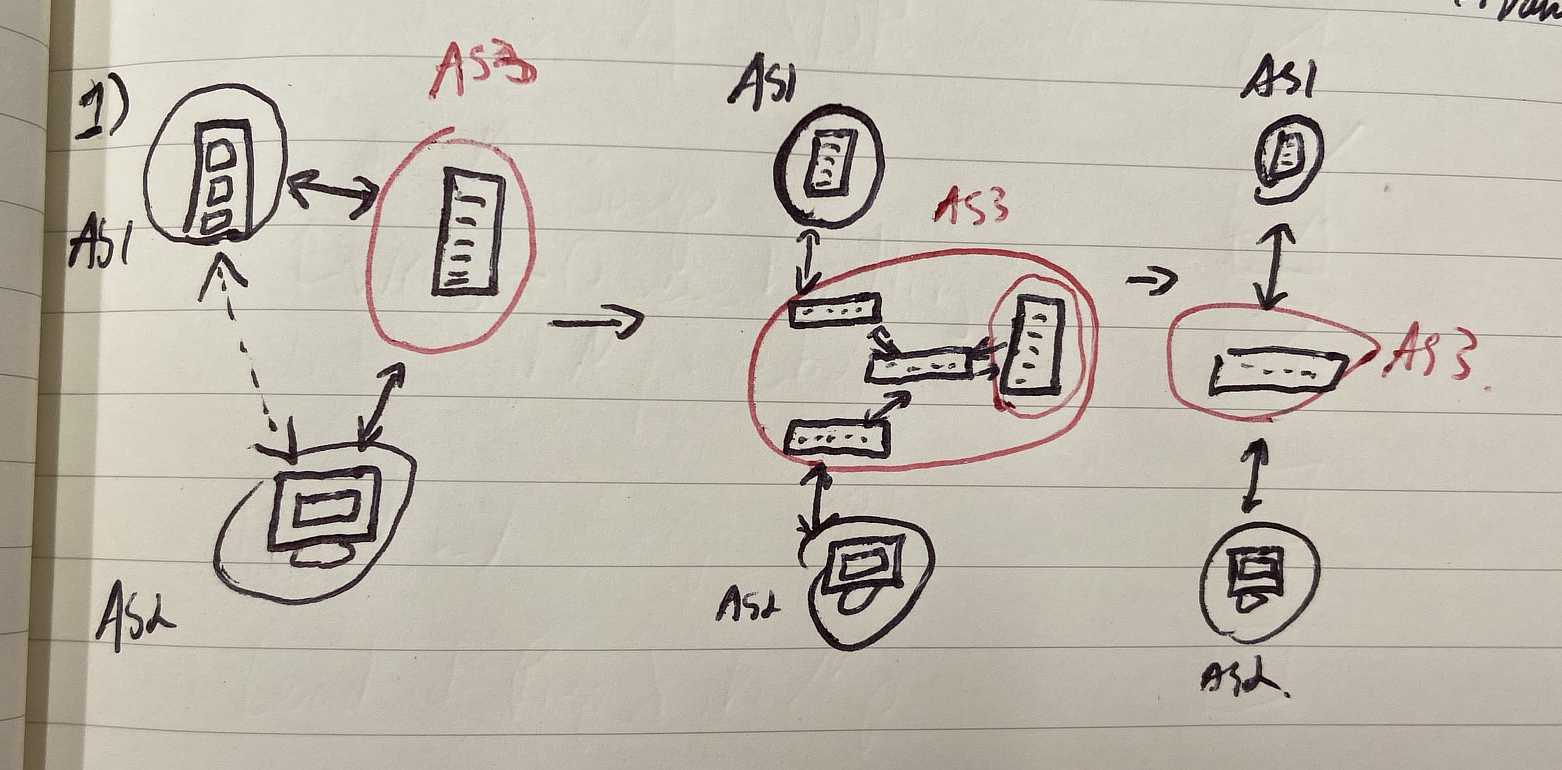
\includegraphics{diagrams/pdp-lit/steering-draft}}
	\caption{text}\label{fig:pdp-lit-steering}
\end{figure}

\begin{figure}
	\resizebox{\linewidth}{!}{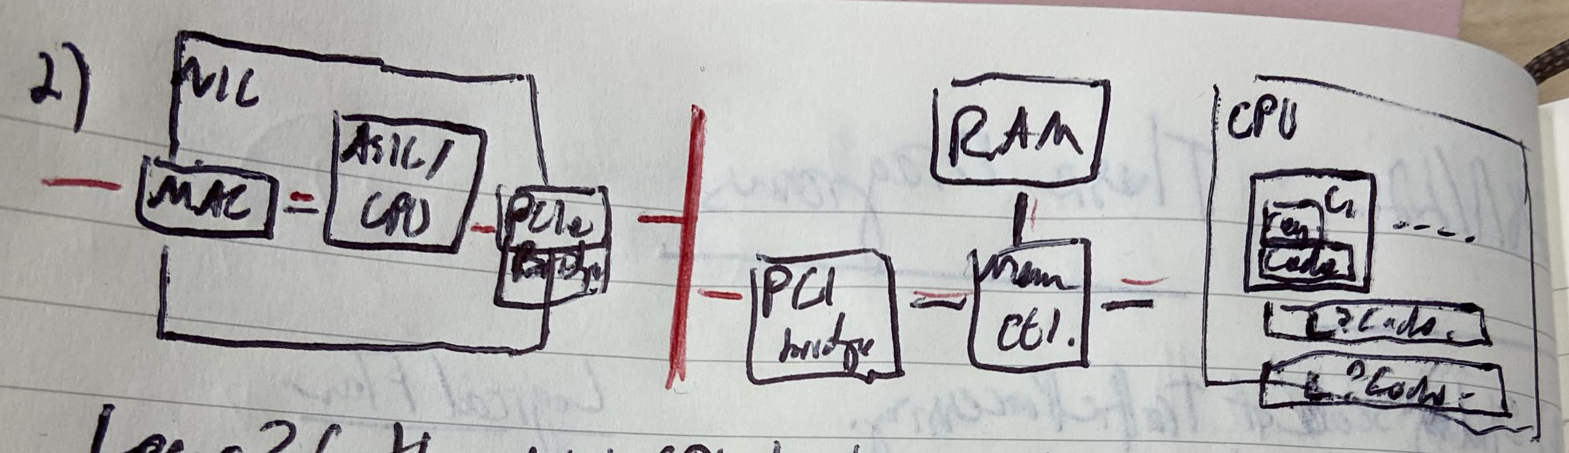
\includegraphics{diagrams/pdp-lit/pci-draft}}
	\caption{text}\label{fig:pdp-lit-pci}
\end{figure}

\begin{figure}
%	\resizebox{\linewidth}{!}{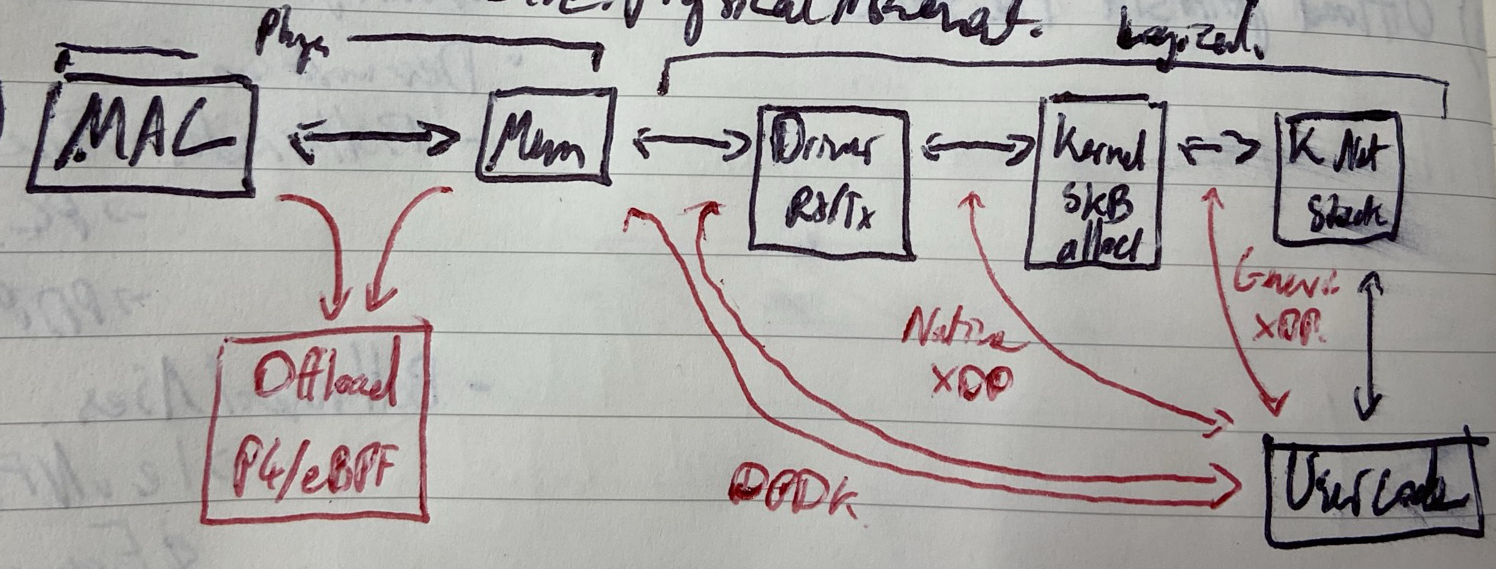
\includegraphics{diagrams/pdp-lit/offloading-draft}}
	\resizebox{\linewidth}{!}{\colorlet{ol-phys}{uofgforest}
\colorlet{ol-log}{uofglavendar}
\colorlet{ol-user}{uofgrust}
\colorlet{ol-userland}{ol-user!75}

\colorlet{ol-arrow}{black}
\colorlet{ol-user-arrow}{ol-user}

\begin{tikzpicture}
	\draw[color=ol-phys,fill=ol-phys!10] (0,0) rectangle ++(2,1) node[pos=.5] (mac) {\gls{acr:mac}};
	\draw[color=ol-phys,fill=ol-phys!10] ($(mac) + (2, -0.5)$) rectangle ++(2,1) node[pos=.5] (nic) {\gls{acr:nic}};
	\draw[color=ol-phys,fill=ol-phys!10,align=center,text=black] ($(nic) + (2, -0.5)$) rectangle ++(2,1) node[pos=.5] (mem) {Memory\\\& Cache};

	\draw[color=ol-log,fill=ol-log!10,align=center,text=black] ($(mem) + (2, -0.5)$) rectangle ++(2,1) node[pos=.5] (rx-tx) {Driver\\Rx/Tx};
	\draw[color=ol-log,fill=ol-log!10,align=center,text=black] ($(rx-tx) + (-1, -2.5)$) rectangle ++(2,1) node[pos=.5] (skb) {Kernel\\\gls{acr:skb} Alloc};
	\draw[color=ol-log,fill=ol-log!10,align=center,text=black] ($(skb) + (-1, -2.5)$) rectangle ++(2,1) node[pos=.5] (ns) {Network\\Stack};

	\draw[color=ol-userland, fill=ol-userland,align=center, text=white, rounded corners] ($(ns) + (-5, -0.5)$) rectangle ++(2,1) node[pos=.5] (userland) {Userland\\Code};

	\draw[color=ol-user, fill=ol-user,align=center,text=white, rounded corners] ($(nic) + (-2, -3.5)$) rectangle ++(2,1) node[pos=.5] (smartnic-offload) {Offload\\C/P4/\glslink{acr:ebpf}{\color{white}eBPF}};

	\draw[color=ol-user, fill=ol-user,align=center,text=white, rounded corners] ($(skb) + (-5, -0.5)$) rectangle ++(2,1) node[pos=.5] (xdp-offload) {Offload\\\glslink{acr:ebpf}{\color{white}eBPF} (\glslink{acr:xdp}{\color{white}XDP})};

	% --------

	\node[color=ol-phys] at (0.75, 1.35) {\large{}Physical};
	\node[color=ol-log, rotate=270] at (11.5, 0.5) {\large{}Logical};

	% --------

	\draw[<->, thick, color=ol-arrow] (mac) -- (nic);
	\draw[<->, thick, color=ol-arrow] (nic) -- (mem);
	\draw[<->, thick, color=ol-arrow] (mem) -- (rx-tx) node[midway, above] {\small{}\glspl{acr:irq}};
	\draw[<->, thick, color=ol-arrow] (rx-tx) -- (skb);
	\draw[<->, thick, color=ol-arrow] (skb) -- (ns);


	\draw[<->, thick, color=ol-user-arrow, shorten >=0.25cm,shorten <=0.3cm] (ns) -- (userland) node[midway, below] {\small{}Socket};
	\draw[<->, thick, color=ol-user-arrow, shorten >=0.12cm,shorten <=0.17cm] (nic) -- (smartnic-offload) node[midway, left, align=center] {\small{}SmartNIC\\Offload};
	\draw[<->, thick, color=ol-user-arrow, shorten >=0.12cm,shorten <=0.12cm] (rx-tx) -- (xdp-offload) node[midway, above, sloped] {\small{}Native \glslink{acr:xdp}{\color{ol-user-arrow}XDP}};
	\draw[<->, thick, color=ol-user-arrow, shorten >=0.05cm,shorten <=0.12cm] (skb) -- (xdp-offload) node[midway, above] {\small{}Generic \glslink{acr:xdp}{\color{ol-user-arrow}XDP}};
	\draw[<->, thick, color=ol-user-arrow, shorten >=0.12cm,shorten <=0.12cm] (userland) -- (xdp-offload) node[midway, right] {\small{}\texttt{AF\_XDP}};

	\draw[<->, thick, color=ol-user-arrow, shorten >=0.12cm,shorten <=0.12cm, out=200,in=150] (mem) to node[left] {\small{}\glslink{acr:dpdk}{\color{ol-user-arrow}DPDK}} (userland);
\end{tikzpicture}}
	\caption[The packet processing stack on host machines, and how the DPDK and XDP frameworks interface with user code.]{The packet processing stack on host machines, and how the \gls{acr:dpdk} and \gls{acr:xdp} frameworks interface with user code. Offload frameworks are useful because they either allow \gls{acr:os} kernel code to be bypassed altogether (\gls{acr:dpdk}), or for packet modification and transmission to be pushed further down the stack (\gls{acr:xdp}). Offloaded \gls{acr:ebpf} user code may typically pass packets to the network stack after some amount of processing, send packets directly back to the \gls{acr:nic} for transmission, or pass packets to user code using a zero-copy mechanism such as \texttt{AF\_XDP}. Crucially, all these mechanisms excise various amounts of processing or imprecise waiting for  interrupts, reducing latencies and increasing packet processing throughput. More details on the logical portion of the stack are presented by \Textcite{DBLP:conf/sigcomm/CaiCVH021}.}\label{fig:pdp-lit-offloading}
\end{figure}

\gls{acr:ebpf}, \gls{acr:xdp}~\parencite{DBLP:conf/conext/Hoiland-Jorgensen18}
?? It should be clear that \gls{acr:ebpf}'s role in the network owes an inestimable debt to \emph{smart packets}.

?? eBPF also allows exec of user code at various points in kernel for instrumentation etc. via \emph{kprobes} and \emph{tracepoints}.

?? Katran~\parencite{katran} L4 load bal;ancer based on \gls{acr:xdp}

?? mention BPFabric~\parencite{DBLP:conf/ancs/JouetP17} somewhere.

later netmap~\parencite{DBLP:conf/usenix/Rizzo12}

?? Morpheus~\parencite{DBLP:conf/asplos/MianoSRRA22} for run-time optimisation.

?? Cool NIC-CPU co-design~\parencite{DBLP:conf/osdi/IbanezMAJ0KM21}

?? Understanding Host Network Stack Overheads~\parencite{DBLP:conf/sigcomm/CaiCVH021}

%\section{Operation and Management}
%
%?? network-network comms? BGP
%
%?? IGP?
%
%?? packets routed on a per-hop basis from their perspective: may be higher level in practice (MPLS, path switching within a gateway)
%
%?? How can we examine this? High-level (above), mid-level ()
%
%?? Two axes: end-to-end protocol and fabric behaviour. interact in a very delicate way (i.e., host )
%
%?? named-data networking as potential structure of the Internet?~\parencite{DBLP:journals/ccr/0001ABJcCPWZ14}
%?? Can I use this to suggest/outline problems which might be solved/encountered in a future Internet?
%
%?? Talk about \gls{acr:as} families here: \glspl{acr:isp}, hypergiants~\parencite{DBLP:conf/sigcomm/GigisCMNKDKS21}...
%?? Data centres: refer to e.g. google Espresso [sigcomm 2017] as big SDN deployments, Jupiter, recent paper too?

%\subsection{Fixed-Function Hardware}
%
%\subsection{Software-Defined Networking}
%
%?? Run through the historical context. Why? What led into P4 (OpenFlow, network operating systems...)
%
%?? \gls{acr:ovs}~\parencite{DBLP:conf/nsdi/PfaffPKJZRGWSSA15} huge here.
%
%?? A survey to mine for stuff~\parencite{DBLP:journals/comsur/NunesMNOT14}
%
%?? Tie into PDP here: active networking and TPP . Think about the concept of protocol boosters~\parencite{DBLP:journals/jsac/FeldmeierMSBMR98}. (NOT READ)

\section{Traffic Characteristics}

?? Can (and should probably) discuss different traffic classes here: congestion-aware, -unaware...

?? Note, explain that this is NOT just TCP vs UDP due to existence of SCTP over UDP (See: DTLS in WebRTC), QUIC over UDP, ...

?? Chain this into \glspl{acr:cca}

?? Explain why you need what.

?? Historical context for their inclusion?

?? Discussion of evolution of traffic: what's come before, what's coming next.
?? Look for older in my old notes, but recent cite here~\parencite{DBLP:conf/anrw/BauerJHBC21}.

?? Describe all my CAIDA analysis here
?? analysis of CAIDA datasets~\parencite{caida-2018-passive}
?? congestion-aware traffic makes up at least \qtyrange{73}{82}{\percent} of packets\sidenote{\url{https://github.com/FelixMcFelix/caida-stats}}
?? Also talk about QUIC's prevalence here

\subsection{Evolution}

\subsection{Emerging Protocols}

?? QUIC~\parencite{DBLP:conf/sigcomm/LangleyRWVKZYKS17}

?? QUIC carries \gls{acr:http} traffic, mostly...

\subsection{Limitations}

\section{Problems in Modern Networks}\label{sec:problems-in-modern-networks}

\subsection{Denial of Service Attacks}
---
?? Normal ones? TCP exhaustion? Application-Level? Sheer bandwidth?

Mirai used as DDoS vector \cite{DBLP:conf/uss/AntonakakisABBB17}.

%?? Big survey \cite{DBLP:conf/imc/JonkerKKRSD17}?
\Textcite{DBLP:conf/imc/JonkerKKRSD17} offer an in-depth analysis and taxonomy of the current landscape of DoS attacks.
They observe that Denial-of-Service is most commonly achieved through \emph{resource exhaustion}---either at the target server or the infrastructure serving it.
Attacks may be classified according to two orthogonal axes: \emph{Direct vs.\ Reflection} and \emph{Volumetric vs.\ Semantic}.
\begin{description}
	\item[Direct] Attackers send packets directly towards their target. Random IP spoofing is often used to make blacklisting more difficult, but leaves evidence of an attack and its characteristics due to \emph{backscatter}, visible to internet telescopes.
	\item[Reflection] Attackers send traffic to a \emph{reflector}, spoofing the source IP of packets to match that of the target. The reflector sends replies to the target, often \emph{amplifying} them in the process.
	\item[Volumetric] DoS is achieved by \emph{resource exhaustion}---CPU or RAM usage at the target host, overfilling transmission buffers along key traffic routes. These are ``service agnostic''.
	\item[Semantic] DoS is achieved by \emph{exploiting program logic}, for instance to crash a target application server. Often tailor-made for a particular service or its deployment environment, such as \emph{Teardrop attacks}.
\end{description}
They find that TCP tends to be the leading transport for direct random-spoofing attacks, while reflection and amplification attacks are dominated by UDP-like protocols (NTP$>$DNS$>$CharGen).
Randomly spoofed direct attacks are found to last longer, and are most intense around ``web ports'' (HTTP, SSH, etc.), evidence is seen to support the existence of ``joint attacks''.
The scale of all attacks is immense, by their measurements: at least a third of the internet is under attack at any one point in time, with at least \num{30000} attacks \emph{visible} each day.

\paragraph{Amplification attacks}
abuse network services with small request bodies and large responses, causing a typically benign service to forward traffic on an attacker's behalf by \emph{reflection}---spoofing the source IP of requests to that of the intended victim.
An attacker requires that the Autonomous System (AS) they belong to doesn't prevent IP spoofing at egress.
In exchange, they are able to split their upstream bandwidth across many reflectors to gain higher volumes of attack traffic from multiple sources without revealing their own IP to the victim.

UDP-based protocols are the typical basis for such attacks, as the transport is connectionless.
While DNS is the most well-known vector for amplification, \textcite{DBLP:conf/ndss/Rossow14} presents an in-depth survey of a wide variety of other vulnerable protocols alongside a rough census of abusable servers.
He examines network services (SNMPv2, NTP, DNS, NetBIOS, SSDP), legacy services (CharGen, QoTD), peer-to-peer networks (BitTorrent, Kad), online games (Steam, Quake 3) and externally abusable botnets (ZAv2, Sality, Gameover).
Scanning for \num{e5} amplifiers of a popular service can be done in minutes, making NTP particularly dangerous due to its high amplification rate.
Furthermore, he notes that the security-focused DNSSEC can exacerbate the problem by the addition of large signatures to message payloads.

\textcite{DBLP:conf/uss/KuhrerHRH14} build further upon this census; they find significant overlap between servers who expose different vulnerable services, connect these services to OS fingerprints, and are able to use DNS proxies to enumerate the ASs who allow IP spoofing.
They find that many eligible reflectors (for i.e., DNS) tend to lie behind dynamic IP addresses and so undergo significant churn (meaning an attacker must often re-scan every few days/weeks).
This is not the case for certain protocols like NTP, where the server list remains far more stable.
The authors also explore the amplification potential of all TCP-based services---given that well-known protocols like HTTP cannot be blocked in most infrastructures, an attacker can abuse retransmissions of the handshake (\texttt{SYN-ACK}) to achieve an amplification factor up to \num{20} if the receiver doesn't send \texttt{RST}.
Differing TCP stacks have varying quirks, so the behaviour of the victim and all reflectors can be hard to predict without prior fingerprinting.
It can be observed that choosing amplifiers of larger geographic distance might increase the amount of \texttt{SYN-ACK} packets in flight before the well-meaning reflector can receive a \texttt{RST}.

NTP quickly became the attack vector of choice \cite{DBLP:conf/imc/CzyzKGPBK14}.
They find that most vulnerable amplifiers are \emph{end-hosts}, typically offering \qty{4}{\times} amplification.
At the time of publication, they observed that NTP amplification attacks had risen in volume by $\sim$\qty{1000}{\times}, though were slowly declining; of particular interest is that \qty{85}{\percent} of attacks over \qty{100}{\giga\bit\per\second} relied upon NTP reflection.
The decrease, they posit, stems mostly from vulnerable servers being patched in response to recent bulletins making the risk very clear to server operators.
How are these patched servers distributed?
They observe that, after the patch period, many of the remaining vulnerable servers are sparsely distributed (rather, the patched servers are clustered under IP blocks).
This is in line with the (un)cleanliness hypothesis put forth by \textcite{DBLP:conf/imc/CollinsSFJWSK07}.
While there were many almost comical findings (a surfeit of NTP servers holding the incorrect time, old versions), of greatest concern was the presence of ``mega-amplifiers'' offering \SIrange{e3}{e9}{\times} amplification due to the presence of network loops.
Over the duration of their study, they observed a \SI{92}{\percent} reduction in abusable IPs, though the uncleanliness observation recurs as the reduction is smaller when considering /24 prefixes (\SI{72}{\percent}).
Regardless, this drop is \emph{far} more significant than any seen in the availability of Open DNS resolvers.
A large part of the remaining vulnerable machines are identified as end hosts, implying that quick fixes are unlikely.
They make it clear that it is hard to reason about who the attackers are (bots, organisers or botmasters), and for what reasons they launch attacks (although ancillary evidence suggests that a remarkably common motivation me be rivalry through, e.g., games).

\Textcite{DBLP:conf/imc/KuhrerHBRH15} investigate the landscape of \emph{open recursive DNS resolvers}, one of the major enabling factors for DNS amplification attacks.
Specifically, a DNS server is said to be \emph{open} if it does not filter requests by source IP address.
The existence of such servers is, they claim, paradoxical: rare is the need to publicly expose recursive DNS resolution when the servers should operate in a well-structured (hierarchical) manner.
By scanning across all IPv4 addresses (according to the methodology of \textcite{DBLP:conf/uss/DurumericWH13}), they discover a downward trend in abusable servers (from \num{26.8e6} to \num{17.8e6} over the year) due to blocked requests/DNS filtering/shutdown/IP churn.
As it turns out, many of these DNS servers run old and vulnerable software, and are very highly represented (\SI{67}{\percent}) by consumer routers linked to dynamic IPs.
Curiously, cache snooping reveals that \SI{61}{\percent} of all open DNS resolvers see active use---many of these resolvers are legit (\SIrange{85}{92}{\percent}), with some even filtering out malicious domains.
The illegitimate set corresponded to censorship in Iran and China, and to malicious redirection to snooping proxies or outright malware.

As of \citeyear{DBLP:conf/imc/JonkerKKRSD17}, the distribution of amplification attacks over UDP protocols was observed to roughly have the pattern (NTP$>$DNS$>$CharGen).
This is in spite of the evidence put forth by \textcite{DBLP:conf/imc/CzyzKGPBK14}, which suggested a decline of NTP-based amplification attacks.
Perhaps the effort to patch up many servers simply hit a (metaphorical) wall of operators who actually cared, thus leaving many viable NTP amplifiers in the wild?

?? Any observations from \textcite{DBLP:conf/raid/KramerKMNKYR15}?

\paragraph{Transit-link attacks}
do some stuff according to these guys \cite{DBLP:conf/sp/SmithS18} (who defend against it), and these guys (who predicted it)---Crossfire \cite{DBLP:conf/sp/KangLG13}, Coremelt \cite{DBLP:conf/esorics/StuderP09}.

\paragraph{Characteristics}

?? Botnet C\&C communication \cite{DBLP:conf/sac/ZandVYK14}? NOT READ

?? \SI{69}{\percent} of targets are web servers \cite{DBLP:conf/imc/JonkerKKRSD17}.

DDoS attacks evolve over timescales of seconds to months.
\Textcite{DBLP:conf/spw/KangGS16} investigate this, and consider the implications and considerations necessary to deal with such occurrences.
Why might attackers desire this?
The authors posit that a diverse attack portfolio makes for more effective attacks, so long as there is \emph{variation}---a single suite or pattern of evolution makes defence (and discovery of the attacker) far simpler.
We see such evolution in:
\begin{description}
	\item[Volume and Capabilities] Peak \SI{300}{\gibi\bit\per\second}$\rightarrow$\SI{600}{\gibi\bit\per\second} over the last 4 years from date of publication.
	\item[Attack targets] E.g., Spamhaus---attackers moved from targeting endpoint servers to targeting the routers in \emph{internet exchange points} (IXPs) once the former was detected.
	\item[Strategy] E.g., semantic attacks $\rightarrow$ volumetric (TCP \texttt{SYN} flood) $\rightarrow$ volumetric (NTP amplification) $\rightarrow$ LFA.
\end{description}
They find that evolution in capabilities occurs over longer timescales, as these typically require resource acquisition (knowledge, bots, etc.).
\emph{Strategies}, however, are easily poised to evolve over short time horizons, typically ``[adapting] to the target's (observed) defensive posture''.
This behaviour was observed in both the cases of SpamHaus and ProtonMail.
In light of this, they suggest a two-tier approach to defence.
To thwart rational adversaries, they suggest the use of \emph{deterrents}---mechanisms located at e.g., a single network point, which can detect attacks and thus increase the cost of maintenance.
Most defences fit this description.
To handle cost-insensitive attackers, they suggest collaborative approaches (such as SENSS \cite{DBLP:conf/acsac/RamanathanMYZ18}).
Unfortunately, the work makes little attempt to describe or study the patterns of short-term evolution which might be expected in a real-world attack.

?? I think we need some other sources to reason about things from a game theoretic perspective---it seems to me that evolution is the name of the game \cite{DBLP:conf/atal/SinhaKT16} (not read this, but seemed relevant at the time).

\paragraph{Amplification}
\textcite{DBLP:conf/ndss/Rossow14}.
?? Inbound/outbound traffic ratios at victim (above a certain bw thres).
?? At the amp, scan activity in surrounding darknets can be an indicator.
?? At the amp, similar ratio analysis (scaled to account for benign activity and real clients who require high bandwidth: lower amp, higher bw).

\textcite{DBLP:conf/imc/CzyzKGPBK14} observe some further hallmarks specific to NTP attacks.
The \texttt{monlist} command principally used as the basis for such attacks can often reveal the list of recent targets after the fact, offering external investigators a means to determine which open NTP servers see active use as amplifiers (and their unwilling victims).
An interesting observation stemming from these records is that the sets of amplifiers and victims are both highly clustered across ASes---individually, that is.
Furthermore, it is observed that attackers choose a selection of target ports on the victim machine (in order of popularity): HTTP, NTP, SSH, gaming services and DNS.
Noting that many of thes services run on \emph{TCP}, it seems likely that attackers are hoping for firewalls to blindly allow through both TCP and UDP on these ports.
Their randomised scanning techniques imply that the culprits behind similar scans could be detected via network telescopes (although it is unclear whether this would reveal the bots, the organiser or the botmaster).

As an aside, the NTP \texttt{monlist} command fragments its $\sim$\SI{50}{\kibi\byte} payload into \SI{482}{\byte} chunks.

\paragraph{Countermeasures}
\textcite{DBLP:conf/ndss/Rossow14}.
?? AS-level---prevent IP spoofing by internal clients.
?? Protocol-level---harden w/ session handling (QUIC, Steam mostly, DTLS) at expense of latency, symmetry of req/resp size, rate limiting resps (limited use).
?? ISP-level---packet filtering on port, len, substring.

?? BGP magic against transit-link attacks and regular \cite{DBLP:conf/sp/SmithS18}.

According to \textcite{DBLP:conf/imc/JonkerKKRSD17}, the most-used techniques in deployment are \emph{DDoS Protection Services}.
While typically proprietary in nature, we see a split between \emph{cloud services}, \emph{in-line systems} (middleboxes) and hybrids thereof.

Cloud services (traffic scrubbers) are known to be most appropriate for handling volumetric attacks and are externally hosted, analysing and filtering out malicious traffic by having services redirect all inbound communication for processing.
The act of redirection is often made cheaper and/or feasible by the use of selective BGP advertisement or DNS modification, aided by reverse proxy or \emph{Generic Routing Encapsulation} (GRE).
Amongst these, BGP-based diversion is most effective where many hosts must be protected, and DNS works most reliably for single-host installations.

In-line systems, hosted within a service's domain of control, are most useful for handling semantic attacks as these often admit \emph{attack signatures} (since they must exploit a particular bug in the server).
Similarly, such attacks tend not to exhibit long-term characteristics that cloud scrubbers might use to aid detection, as many of these attacks present themselves as a single packet.

These authors further find that being attacked does not necessarily increase the likelihood of moving to a DPS---what is an effective indicator is the \emph{strength} of attack targeting a particular service.
To explain, around a fifth of targets already had a DPS prior to an attack, and only \SI{4}{\percent} of victims without a DPS migrate to one.

\Textcite{DBLP:conf/lcn/BragaMP10} have examined the detection of ongoing (flooding-based) DDoS attacks through \emph{self-organising maps}, making use of SDN to gather statistics effectively.
Many of their features aren't overly relevant, as their focus is not active defence or discovering \emph{which} hosts are contributing to an attack.

?? AmpPot \cite{DBLP:conf/raid/KramerKMNKYR15}

\emph{SPIFFY} \cite{DBLP:conf/ndss/KangGS16} aims to remedy transit-link attacks by observing how flows from each source respond to a sudden increase in available bandwidth.
\Citeauthor{DBLP:conf/ndss/KangGS16} realise that bots participating in an attack are often unable to match this bandwidth expansion due to having already saturated the capacity of their outbound links, while legitimate flows typically speed up to match the new fair-share rate.
%Attackers must either be detected or reduce the throughput of each bot, increasing the cost of launching an attack.
Unlike our approach (and due to the class of attacks it is designed to defend against), SPIFFY is intended to be deployed within ISP networks, although some of our feature choices are backed by similar observations.
?? Flaws? what can't it do that we can do better? Long times to compute TBE routes on real networks, low expansion factor in real network can require more ``rounds'' of filtering. (``takes only'' \SI{14}{\second} for Cogent network? gross.)
?? I believe their assumptions may not extend to CBR traffic (e.g., UDP VoIP traffic), which we know makes up a sizeable proportion of network traffic.

\emph{Athena} \cite{DBLP:conf/dsn/LeeKSPY17} is a more generalised SDN framework for intrusion detection, but has shown the use of a \emph{k-nearest neighbours} classifier to detect individual attack flows.
Although heavyweight (and proven to be effective compared with \textcite{DBLP:conf/lcn/BragaMP10}), their comparison against SPIFFY lacks the quantitative evidence required to understand how the system compares.

SENSS \cite{DBLP:conf/acsac/RamanathanMYZ18} aims to help hosts and/or \emph{endpoint-servers} communicate upstream with ISPs.
The rationale is that, although DDoS traffic can be filtered at any point along its path it will impact less of the network if it is filtered \emph{close to its source}---this observation holds true in all attack classes (direct, reflection, LFA/crossfire), which exhibit a tree-like pattern of traffic.
This information currently propagates through human channels, eventually leading to traffic black-holing being performed by key ASes.
The core idea is that the \emph{victim} should be given responsibility for intelligence and decision-making, who pass on their requests to ISPs (alongside ample payment)---they are able to show that this approach functions for multiple algorithms.
The need for payment does seem odd at the outset, but it becomes clear that this is a necessary mechanism to enable ``remote networks to collaborate on demand, without prior trust''.
While all the software engineering work seems well-considered, it appears to hinge on the condition that HTTP/TCP sessions can be reliably held over the saturation zone between high-priority endpoints---they do admit that alternative channels may be possible through elected proxies or UDP-based mechanisms like DOTS \cite{ietf-dots-use-cases-17}.
The mitigation strategies they propose do hold water, and strike me as interesting---using NAT for true outbound requests as a mechanism for reflector filtering close-to-source, similar techniques to others to ``route around'' the congestion added by LFAs, and location-based filtering for signature-free attacks.
What I'm concerned about is the degree of collaboration required; it seems likely to me that there may exist e.g., amplifiers who are difficult to block in such a manner due to non-cooperative ASes on their path, with geography and network uncleanliness as contributing factors...
Their evaluation is convincing---a mixture of a testbed experiment over a small-scale environment (Iperf + ``custom UDP flood'') and an AS-level simulation recreating the DDoS attack on Dyn (gravity model \cite{DBLP:journals/ccr/Roughan05}, cogent topology from Topology Zoo \cite{topology-zoo}).

?? Collaborative soln (?) \cite{DBLP:journals/tnsm/SimpsonSMJPH18}

\Textcite{DBLP:conf/sp/SmithS18} present techniques based on AS-level routing to tackle both transit-link and flooding-based attacks.
This view is taken due to the perceived cost of per-stream classification and inherent sensitivity to adversarial examples or crafted input.
The approach is creative, relying upon BGP \emph{fraudulent route reverse poisoning} to preserve traffic to a target AS, but unlike SPIFFY the approach doesn't actually \emph{remove} the congestion.
Because of this, traditional flooding-based attacks aren't fully alleviated.

?? DDoS Open Threat Signalling \cite{ietf-dots-use-cases-17} as an architecture to maybe enable the deployment of many of these?

\subsection{Scaling}

\subsection{Fairness}

%\section{Programmable Data-Planes}
%
%?? 2021 --- crucial to sell the why! What can be gained moving to this level, new state measures enable new applications, in-nic/switch exec reduces latencies, increases throughputs, etc...
%?? Probably want a worked example showing how in-network compute helps. I.e., network graph, show processing at nodes
%
%?? Explain \gls{acr:npu} here...
%
%?? Understanding Host Network Stack Overheads~\parencite{DBLP:conf/sigcomm/CaiCVH021}
%
%?? Evidence of deployment in real, huge transit networks~\sidenote{\url{https://wiki.geant.org/display/RARE/Home}, \url{https://wiki.geant.org/display/NETDEV}}
%
%?? arbitrarily reconfigurable hardware located directly on the data path
%
%?? OvS?~\parencite{DBLP:conf/sigcomm/TuWAP21}

%?? Understanding Host Network Stack Overheads~\parencite{DBLP:conf/sigcomm/CaiCVH021}
%?? mention how it came to this: this was an alternate solution to latency or throughput concerns which plague VNF approaches as they scale (see Metron~\parencite{DBLP:conf/nsdi/KatsikasBKSM18} paper for good discussion of RSS, etc., which solve these problems in their own way)
%
%?? new ways to implement stateful + stateless packet processing.
%
%?? History? RMT~\parencite{DBLP:conf/sigcomm/BosshartGKVMIMH13}, ClickNP, GPU offload papers. See Metron paper for cites.
%
%?? NetFPGA~\parencite{DBLP:conf/fpga/IbanezBMZ19}
%
%?? Getting even faster?~\parencite{nokia-fp5}

%\section{Control and Management}
%
%?? Refer back to History through OpenFlow -- what prompted the evolution?
%
%?? Control of these devices has a lot in common with OpenFlow -- controller, except using commodity hardware to install firmwares, and so on,

%\section{Software Frameworks}
%
%\subsection{eBPF}
%?? eBPF
%
%?? BPFabric
%
%\subsection{P4}
%?? P4
%
%?? Others who lost?
%
%?? How do these differ? What do they share?
%
%?? Popular frameworks now support this -- ONOS, eBPF translators, behavioural model software switch...
%
%?? Things like Lucid built on top of P4?~\parencite{DBLP:conf/sigcomm/SonchackLRW21}
%
%?? P4~\parencite{DBLP:journals/ccr/BosshartDGIMRSTVVW14} and \emph{programmable dataplane} (PDP) hardware~\parencite{DBLP:journals/micro/ZilbermanACM14, netronome-smartnic, xilinx-alveo, barefoot-intel}
%
%?? Cool NIC-CPU co-design~\parencite{DBLP:conf/osdi/IbanezMAJ0KM21}
%
%\fakepara{PDP design for asynchronous compute}
%\emph{PANIC}~\parencite{DBLP:conf/hotnets/StephensAS18} places a routing fabric between distinct packet/data processing elements \emph{in a SmartNIC}.
%Such designs would enable general, asynchronous, and novel compute in SmartNICs and switches, for instance offering consistent and easy to use communication between workers versus hard-coded ME relationships.
%Event-driven versions of P4 have been suggested~\parencite{DBLP:conf/hotnets/IbanezABM19}.
%Timer events and device state changes would empower in-network RL use-cases, signalling timesteps for RL agents or new, effective, fine-grained sources of input state.

\section{Offloading frameworks}
\emph{ClickNP}~\parencite{DBLP:conf/sigcomm/LiTLPLXXC16} targets NetFPGAs: DAG of predefined Click-like blocks, i.e. VHDL segments.
Why?
The C$\rightarrow$VHDL pipeline leads to awful code, so this achieves better FPGA usage.

\emph{Floem}~\parencite{DBLP:conf/osdi/PhothilimthanaL18} presents a DSL in python, which compiles to C for host and specific target NIC.
This does require specific dev effort per-target-NIC.

\emph{iPipe}~\parencite{DBLP:conf/sigcomm/LiuCSKPG19} runs C language programs on SmartNIC (intended) and host (emergency) according to whether traffic is at-risk of suffering from SmartNIC resource contention.
Processing is dynamically `unoffloaded' back to the host machine if SmartNIC load is too great.
This requires identical language support on both accelerator and host---which is very much not guaranteed.

\emph{hXDP}~\parencite{DBLP:conf/osdi/BrunellaBBPSBCP20} allows eBPF execution on FPGA---supports expanded eBPF ISA rather than converting program into a complete pipelined circuit (i.e., this runs as a coprocessor).
Why?
Fast redesign/reinstall time: a complete circuit bake takes ages, while JITing and compiling an eBPF program into their new ISA is pretty fast.
This includes some very cool details on around VLIW instruction-level parallelism built into their ISA and figured out during compile-time.

\emph{Gallium}~\parencite{DBLP:conf/sigcomm/ZhangZK20} converts a C++ (ClickNF program)$\rightarrow$auto-leverage PDP (P4 + C++ + P4).
Split into pre- and post-host P4 segments, with a host C++ program.
Gallium uses LLVM IR to determine read-write dependencies between variables/basic-blocks, account for PDP capabilities of packet reads (i.e., PDP can't touch packet body past $\sim$\qty{300}{\byte}), can move about \qty{100}{\byte} metadata between sites.
Identifies fast/slow paths if offloading can be elided.
Main drawback is that some annotation needed to translate Click primitives into MATs etc., otherwise the conversion to P4 means minimal additional work per target accelerator.

\emph{Flightplan}~\parencite{DBLP:conf/nsdi/SultanaSGPHSBDL21} splits P4 program into subchunks placed and routed between \{PDP, FPGA, host, server, NPU, ASIC\} for pipelining (i.e., performance) or redundancy.
Their disaggregation inserts blocks before and after splits to handle metadata (state) passing.
Their compiler breaks the programs on basic blocks with user annotations, where specific implementations manually given for some \texttt{extern}s to enable device-specific acceleration.
Data dependencies between basic blocks are extracted from the P4 IR in P4C compiler.

Preliminary work on splitting eBPF programs between an XDP part and userland part has been proposed~\parencite{DBLP:conf/conext/ShahinfarMSSBA21}.
This considers both horizontal (i.e., chunks in driver with XDP tail-calls) or vertical (user$\leftrightarrow$kernel) splits of code.
I think their XDP vs.~AF\_XDP split test confirms that the first handler in the XDP hook is basically single-threaded, which probably has some implications for our use of it as an offload.

%\paragraph{Misc P4 translations.}
%T4P4S~\parencite{DBLP:conf/hpsr/VorosHKLTL18} converts P4 programs into C, which are linked against a target-specific network hardware abstraction layer.
%This seems to be the most effective host deployment for P4 at the moment, since it buys you DPDK-capable P4 dataplane installation compared to how terribly slow BMv2 is known to be.
%Slower than native DPDK, but outpaces OvS, and allows definition of HAL binaries in SmartNIC C code as needed too.
%
%$\mu$P4~\parencite{DBLP:conf/sigcomm/SoniR0DF20} extends P4C to decompose parser and action code into independent subprograms, to simplify porting behaviours between different switch models (V1Model, PSA, SUME, ...).
%
%Lyra~\parencite{DBLP:conf/sigcomm/GaoZLMZTSCZY20} is a language for running Network Programming Language friendly programs (i.e., same constraints as P4 programs) across heterogeneous switch hardware, plus placement constraints.
%
%?? P4 Verification~\parencite{DBLP:conf/sigcomm/TianGLZCZDYMTLW21}---also shows use of \gls{acr:pdp} switches in real large-scale networks (\gls{acr:isp}?)

\section{Use Cases}

?? On-switch (Tofino) DDoS detection and defence~\parencite{DBLP:conf/uss/LiuNNLK0BYS21}

\subsection{In-Network Computation}\label{sec:in-network-computation}
?? In-network computation.\sidenote{Test text hello.}

iSwitch~\cite{DBLP:conf/isca/LiLYCSH19} uses programmable switches to combine model updates between RL agents acting as part of a distributed RL training system.
Note that we discuss this in section \ref{sec:wtf}.\sidenote{Make sure that this is properly explained in the PDP seciton: source is `report-yr2.tex'.}

?? A recent line of research in the community has been to investigate \emph{Binarised/Bitwise Neural Networks} (BNNs)~\parencite{DBLP:conf/nips/HubaraCSEB16,DBLP:journals/corr/KimS16,DBLP:journals/corr/MiyashitaLM16} for line-rate packet classification.
?? \emph{BaNaNa SPLIT} shows this as an offload mechanism~\parencite{DBLP:conf/sigcomm/SanvitoSB18,DBLP:journals/corr/abs-1801-05731}; DNN inference is often carried out on the \emph{CPU} to reduce latency imposed by GPU batching and transfer, but fully-connected layers can be accelerated further by NICs.

\subsection{Network Telemetry}
?? Others (try to avoid DDN cases here).

?? The P4 ecosystem already presents novel, openly-available, fine-grained traffic measurement techniques that can be installed and controlled with ease~\parencite{DBLP:conf/sigcomm/GuptaHCFRW18,DBLP:conf/sigcomm/ChenFKRR18,DBLP:conf/sosr/GhasemiBR17}

\subsection{Transport Layer Optimisation}
?? Hi~\parencite{DBLP:conf/nsdi/ArashlooLGRWW20} Network stacks being moved into NICs to reduce latency/CPU utilisation, mainly for datacentre use-cases---otherwise, \SI{100}{\giga\bit\per\second} can't be hit. New API \emph{Tonic} for transport layer in user code (send, data management), DMA to NIC and let it handle all (de)packetisation. ``Transport logic'' goes to Tonic. Main design is datacentres, so not very high BDPs (long-fat) $\rightarrow$ \si{\kilo\byte} inflight data.

\subsection{Active Queue Management}
Turns out that you can't just write it in P4, you need to co-design for the target environment---with meaningful performance cost to boot, based on the tradeoffs you need to make~\parencite{Kunze-P4-AQM}.

\subsection{KV Stores}
NetChain~\parencite{DBLP:conf/nsdi/JinLZFLSKS18}.

\subsection{ML in PDP}
?? ML in the dataplane~\parencite{DBLP:conf/hotnets/XiongZ19,DBLP:conf/sigcomm/SanvitoSB18,DBLP:journals/corr/abs-1801-05731,DBLP:journals/corr/abs-2009-02353,langlet-ml-netronome,DBLP:journals/corr/abs-2002-08987}

%\section{Hardware Designs}
%
%?? Mention FPGA vs many-core
%
%?? P4 etc. can actually all run on commodity hardware, which offers a third (suboptimal) hardware class.
%
%?? Ref the paper that Haruna presented \parencite{DBLP:conf/icc/MafiolettikDMRV20}: pareto front of work-division optimality for SmartNICs (i.e., addition of high-latency cores).
%
%?? How do these limit and influence what code can be run on different device classes? The time taken to adapt the network?
%
%\subsection{Models of Parallelism}
%
%\subsection{Flexibility}
%
%\subsection{Mapping Software Frameworks}

\section{Summary}
Eh.
